\documentclass[a4paper,12pt,oneside,top=6cm,bottom=3cm,left=3.5cm,right=3.5cm,openright,reqno,table]{book}
\usepackage[english, italian]{babel} 
\usepackage{microtype}
\usepackage[utf8]{inputenc}
\usepackage{subfigure}
\usepackage{epsfig}
\usepackage{amsmath, amssymb}
\usepackage[linesnumbered,lined,commentsnumbered,italiano]{algorithm2e}
\usepackage{fancybox}
\usepackage{listings}
\usepackage{url}
\usepackage{graphicx}
\setlength{\marginparwidth} {2cm}
\renewcommand{\baselinestretch}{1.3} 
\usepackage{todonotes}
\usepackage{moreverb}
\usepackage{multirow}
\usepackage{multicol}
\usepackage[labelfont=it,textfont={it}]{caption}
\usepackage[final,bookmarks,breaklinks,colorlinks,allcolors=black]{hyperref}
\usepackage{soul,color}
\usepackage[block=ragged,backend=biber,natbib=true,style=ieee]{biblatex} % Use the bibtex backend with the author year citation style (which resembles APA)

\addbibresource{bibliography.bib} % The filename of the bibliography
\usepackage[autostyle=true]{csquotes} % Required to generate language-dependent quotes in the bibliography
\newcommand{\wip}[1]{\todo[inline,color=yellow!20!white]{\textbf{WIP:} #1}}
\newcommand{\done}[1]{\todo[inline,color=green!20!white]{\textbf{Done:} #1}}
\newcommand{\todoi}[1]{\todo[inline]{\textbf{Todo:} #1}}

\newcommand{\eg}{\textit{e}.\textit{g}., }

\newcommand{\ie}{ \textit{i}.\textit{e}., }
\definecolor{gibgray}{rgb}{0.898, 0.898, 0.898}

\newenvironment{rqbox}{\par\begingroup
	\setlength{\fboxsep}{5pt}\findlength
	\setbox0=\vbox\bgroup\noindent
	\hsize=0.95\linewidth
	\begin{minipage}{0.95\linewidth}\normalsize}
	{\end{minipage}\egroup
	\textcolor{black}{\fboxsep1.5pt\fbox
		{\fboxsep5pt\colorbox{gibgray}{\normalcolor\box0}}
		}
	% \endgroup\par\addvspace{6pt minus 3pt}\noindent
	\endgroup\par\noindent
	\normalcolor\ignorespacesafterend
	}
\let\Examplebox\examplebox
\let\endExamplebox\endexamplebox



\definecolor{mygreen}{rgb}{0,0.6,0}
\definecolor{mygray}{rgb}{0.5,0.5,0.5}
\definecolor{mymauve}{rgb}{0.58,0,0.82}
\definecolor{pblue}{rgb}{0.13,0.13,1}
\definecolor{pgreen}{rgb}{0,0.5,0}
\definecolor{pred}{rgb}{0.9,0,0}
\definecolor{pgrey}{rgb}{0.46,0.45,0.48}
\definecolor{codebackground}{rgb}{0.95, 0.95, 0.92}
\definecolor{gray50}{gray}{.5}
\definecolor{gray40}{gray}{.6}
\definecolor{gray30}{gray}{.7}
\definecolor{gray20}{gray}{.8}
\definecolor{gray10}{gray}{.9}
\definecolor{gray05}{gray}{.95}
\definecolor{arsenic}{rgb}{0.23, 0.27, 0.29}
\definecolor{arsenic}{rgb}{0.23, 0.27, 0.29}
\lstset{ %
	backgroundcolor=\color{white},   % choose the background color; you must add \usepackage{color} or \usepackage{xcolor}; should come as last argument
	basicstyle=\footnotesize,        % the size of the fonts that are used for the code
	breakatwhitespace=false,         % sets if automatic breaks should only happen at whitespace
	breaklines=true,                 % sets automatic line breaking
	captionpos=b,                    % sets the caption-position to bottom
	commentstyle=\color{mygreen},    % comment style
	deletekeywords={...},            % if you want to delete keywords from the given language
	escapeinside={\%*}{*)},          % if you want to add LaTeX within your code
	extendedchars=true,              % lets you use non-ASCII characters; for 8-bits encodings only, does not work with UTF-8
	frame=single,
	keepspaces=true,                 % keeps spaces in text, useful for keeping indentation of code (possibly needs columns=flexible)
	keywordstyle=\color{blue},       % keyword style
	morekeywords={*,...},            % if you want to add more keywords to the set
	numbers=left,                    % where to put the line-numbers; possible values are (none, left, right)
	numberstyle=\tiny\color{mygray}, % the style that is used for the line-numbers
	rulecolor=\color{black},         % if not set, the frame-color may be changed on line-breaks within not-black text (e.g. comments (green here))
	showspaces=false,                % show spaces everywhere adding particular underscores; it overrides 'showstringspaces'
	showstringspaces=false,          % underline spaces within strings only
	showtabs=false,                  % show tabs within strings adding particular underscores
	stringstyle=\color{mymauve},     % string literal style
	tabsize=2,	                   % sets default tabsize to 2 spaces
	title=\lstname                   % show the filename of files included with \lstinputlisting; also try caption instead of title
}
%%%%%%%%%%%%%
\definecolor{gray}{rgb}{0.4,0.4,0.4}
\definecolor{darkblue}{rgb}{0.0,0.0,0.6}
\definecolor{cyan}{rgb}{0.0,0.6,0.6}


\definecolor{javared}{rgb}{0.6,0,0} % for strings
\definecolor{javagreen}{rgb}{0.25,0.5,0.35} % comments
\definecolor{javapurple}{rgb}{0.5,0,0.35} % keywords
\definecolor{javadocblue}{rgb}{0.25,0.35,0.75} % javadoc

%%%%%%%%%%%%%%%%%%%%%%%%

%%%%%%%%%%%
%SUMMARY BOX

\newcommand\rf[1]{\textcolor{black}{#1}}
\RequirePackage{fontawesome}

\newcommand{\keyfindingsrqa}[1]{ %
	\vspace{5pt} %
	\noindent\fcolorbox{arsenic}{gray10}{%
		\parbox{0.97\linewidth}{% 
			\textbf{\faKey\ Stato dell'arte} #1 %
		}%
	}%
	\vspace{5pt} %
}%
\newcommand{\keyfindingsrqb}[1]{ %
	\vspace{5pt} %
	\noindent\fcolorbox{arsenic}{gray10}{%
		\parbox{0.97\linewidth}{% 
			\textbf{\faKey\ Percezione degli sviluppatori} #1 %
		}%
	}%
	\vspace{5pt} %
}%

%%%%%%%%%%%%%%%%%%%%%%%%%%%%
\begin{document}
\selectlanguage{italian}
\begin{titlepage}
\begin{center}
{\Large Universit\`a degli Studi di Salerno}\\[0.2truecm]
{\large Dipartimento di Informatica}\\

\hrulefill\\
\vspace{0.5cm}

\epsfig{file=Figure/unisa.pdf,width=4truecm}\\[0.2truecm]
\vspace{0.5cm}
{\Large Tesi di Laurea Magistrale in }\\[0.2truecm]
{\Large Informatica}\\
\vspace{3cm}
{\huge Technical Debt in }\\[0.2truecm]
{\huge Sistemi di Intelligenza Artificiale:}\break
{\huge uno Studio Empirico sullo Stato dell'Arte e della Pratica}\\
\vfill

{\bf Relatore} \hfill {\bf Candidato}\ \ \\
Prof. Fabio Palomba \hfill Gilberto Recupito\\
    \hfill Matricola:0522500842

\hrulefill 

Anno Accademico 2021-2022

\end{center}
\end{titlepage}
\pagenumbering{roman}
\clearpage
\vfill
\hfill \textit{A mio padre e mio fratello.}
\chapter*{Abstract}
La diffusione dell'intelligenza artificiale (AI) nei prodotti industriali ha condotto alla creazione di sistemi in continua crescita, portando alla trasformazione di modelli sperimentali in prodotti commerciali.
L'esigenza di favorire l'evoluzione di questi sistemi ha portato all'introduzione delle pratiche di ingegneria del software mirate ai sistemi di intelligenza artificiale.
In particolare, la necessità di preservare la qualità dei modelli AI ha incrementato l'interesse della ricerca e dell'industria nel trovare metodologie utili a affrontare le più diffuse minacce alla qualità di questi sistemi.
In questo contesto, lo studio e le analisi di prevenzione delle tipologie di Technical Debt specifiche per AI (AI Technical Debt) rappresenta attualmente una delle più grandi sfide, in quanto la gestione di esse consente di identificare e mitigare severe problematiche che influenzano diversi aspetti di qualità dei sistemi.
Mentre l'importanza di gestire AI Technical Debt è emergente, l'attuale sforzo della ricerca e dell'industria non è sufficiente a fornire una ben definita tassonomia e catalogazione delle istanze che possono causare AI Technical Debt nei sistemi AI.
Il lavoro di tesi definito, quindi, fornisce un cospicuo contributo alla definizione delle istanze di AI Technical Debt, offrendo alla comunità accademica e industriale di poter analizzare la frequenza, la severità e l'impatto sugli aspetti di qualità delle possibili minacce che impediscono l'evoluzione dei moduli AI all'interno dei sistemi.
Di conseguenza, è stato condotto uno studio preliminare della letteratura presente nello stato dell'arte, al fine di estrarre le tipologie e le istanze di AI Technical Debt più diffuse.
Successivamente, il lavoro di tesi presenta l'investigazione del punto di vista di 54 professionisti di sistemi AI sulla frequenza, severità e impatto di istanze che possono causare AI Technical Debt sulla struttura del codice e sull'architettura del sistema.
I risultati mostrano un'alta diffusione e discussione in letteratura delle istanze di AI Technical Debt relative ai dati (\textit{data debt}), in particolare per le istanze che identificano dipendenze instabili tra i dati e le istanze che identificano informazioni e dati poco utilizzati dal modello.
I risultati estratti sia dallo stato dell'arte che dalla pratica evidenziano, inoltre, un'alta influenza delle istanze di AI Technical Debt relative al codice (\textit{code debt}) e all'architettura (\textit{architectural debt}).
In particolare, le istanze di \textit{Undeclared Consumers}, \textit{Pipeline Jungle} e \textit{Jumbled Model Architecture} sono state identificate essere tra le più severe e conseguire in un alto impatto nella qualità dei sistemi AI.


\vfill
\tableofcontents

\pagenumbering{arabic}
%%%%%%%%%%%%%%%%%%%%%%%%%%%%
\chapter{Introduzione}
% devono seguire solo il primo capitolo
\phantomsection
%\addcontentsline{toc}{chapter}{Introduzione}
\chapter{Introduzione}
\markboth{Introduzione}{}
% [titolo ridotto se non ci dovesse stare] {titolo completo}

\section{Motivazioni e Obiettivi} %\label{1sec:scopo}

\section{Risultati}

\section{Struttura della tesi}

 
%%%%%%%%%%%%%%%%%%%%%%%%%%%%
\chapter{Background}

In questo capitolo sono illustrate le nozioni preliminari che forniscono una base solida al presente lavoro di tesi.


\section{Qualità del Software}
Le tecniche di Ingegneria del Software sono fondamentali alla gestione della qualità del software AI.
%questo rovina pure la pagina quindi non preoccuparti
Lo standard IEEE definisce l'ingegneria del software come l'applicazione di un approccio sistematico, disciplinato e quantificabile volto allo sviluppo e la manutenzione del software \cite{IEEE610}.
L'insieme delle metodologie, i principi e le tecniche di Ingegneria del software hanno l'obiettivo di ottenere un prodotto software affidabile ed efficiente.

L'insieme delle attività che definiscono le fasi di realizzazione del software, a partire dalla definizione della sua specifica fino alla manutenzione viene definito processo di ciclo di vita del software.
Esistono diversi processi di cicli di vita del software altamente adoperati all'interno del settore industriale, e tutti i processi esistenti includono le seguenti fasi \cite{Sommerville}:

\begin{itemize}
    \item \textbf{Specifica del software}: insieme delle attività di comprensione e definizione delle specifiche richieste dal sistema e l'identificazione dei vincoli sulle operazioni e lo sviluppo del sistema.
    
    \item \textbf{Progettazione e implementazione del software}: insieme delle attività volte alla progettazione dell'architettura, delle interfacce e delle componenti.
    
    \item \textbf{Validazione del software}: insieme delle attività che effettuano la validazione e la verifica del software, includendo sia attività di ispezione e di revisione del software, sia attività di testing.
    
    \item \textbf{Evoluzione del software}: insieme delle attività che consentono il continuo aggiornamento e favorire la crescita dinamica del software.
    
\end{itemize}
Ognuna di queste fasi prevede una serie di attività utili al supporto della realizzazione del progetto. In particolare, è necessario notare che ogni fase viene supportata da attività di pianificazione del progetto, di monitoraggio e di tracciabilità degli artefatti.
Una delle più importanti attività che viene svolta durante la fase di monitoraggio del sistema software è la valutazione della qualità.

Una definizione importante e precisa da considerare quando si interagisce con la qualità del software è quella definita dallo Standard ISO/IEC 25010:2011 \cite{ieee25010}.
Essa viene definita come \textit{"la capacità del software di soddisfare le esigenze dichiarate e implicite sotto specifiche condizioni quando utilizzato"}.
Queste particolari esigenze da soddisfare sono state definite dai modelli di qualità, i quali hanno lo scopo di effettuare una categorizzazione della qualità del software tramite un'insieme di caratteristiche.
Successivamente queste caratteristiche sono ulteriormente scomposte ciclicamente in sottocaratteristiche e proprietà.
Ogni definizione di sottoinsieme di caratteristiche ha lo scopo di poter ottenere una rappresentazione dettagliata di un aspetto della qualità del software, a tal punto da renderlo misurabile. In figura \ref{fig:quality_model_def} è possibile osservare come dalla definizione generica di un aspetto della qualità del software è possibile quindi andare a definire delle proprietà che sono direttamente misurabili.
\begin{figure}[h]
    \centering
    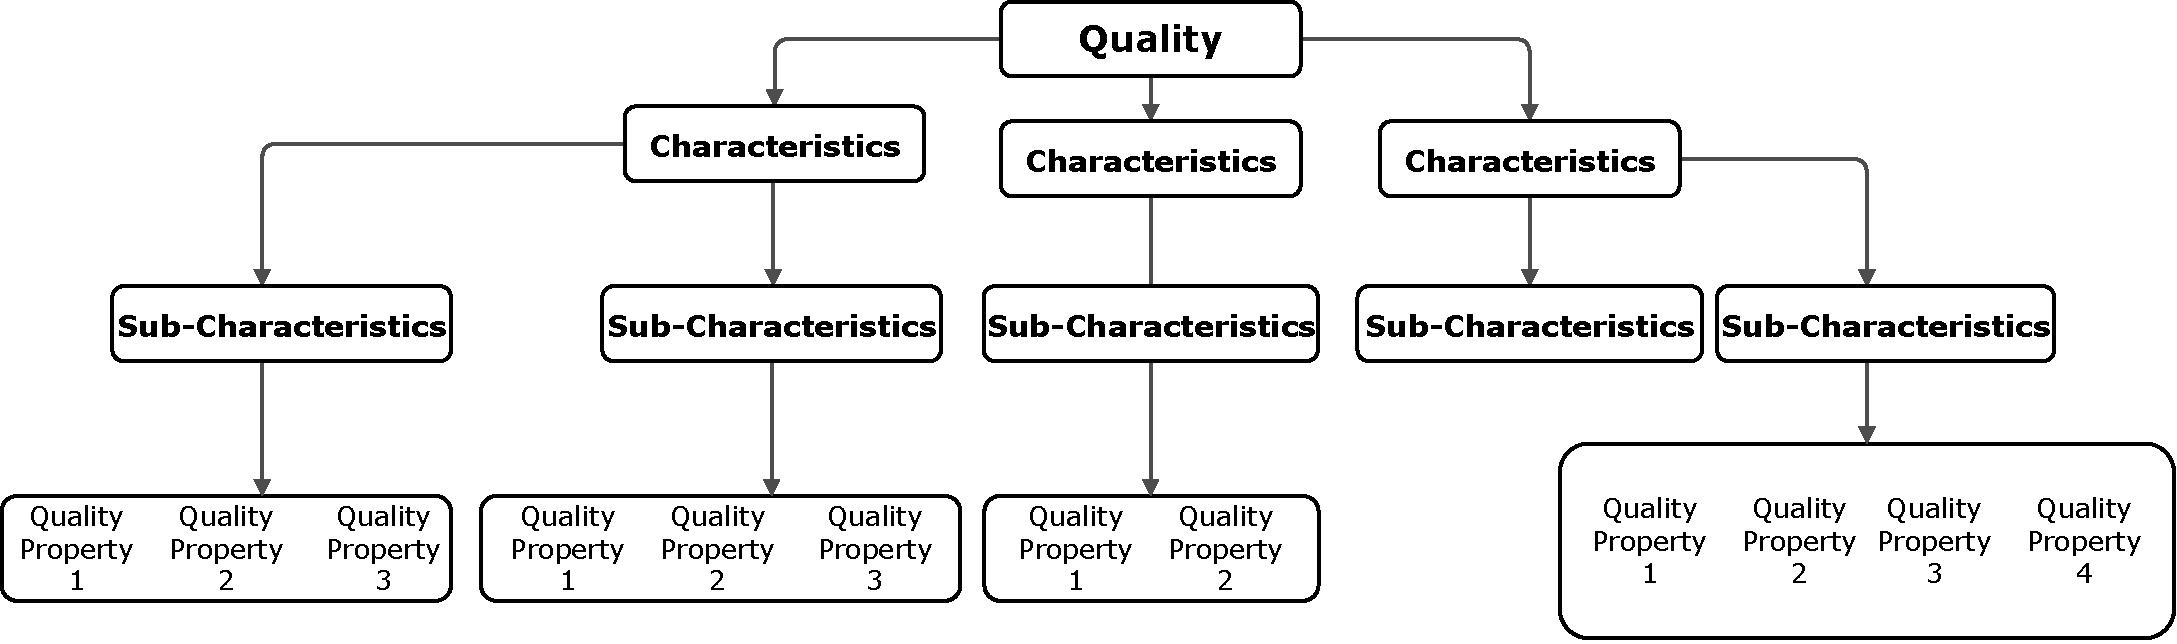
\includegraphics[width=1\textwidth]{Figure/Background/quality_def.pdf}
    \caption{Struttura utilizzata per la definizione di modelli di qualità}
    \label{fig:quality_model_def}
\end{figure}

Tra i modelli maggiormente utilizzati per la gestione della qualità del software è presente il modello ISO/IEC 9126.
%continuare con la definizione tramite ref mendeley isoiec 9126

\subsection{ISO/IEC 9126}
Le norme proposte all'interno del modello \textit{ISO/IEC 9126} sono emesse dall'ISO, l'organismo internazionale di standardizzazione (International Organization for Standardization) e, in particolare, dall'organo interno del settore delle tecnologie e della comunicazione (IEC, International Electrotechnical Commission).
Le norme emesse quindi definiscono la qualità del software in quattro parti: 
\begin{enumerate}
    \item Modello di qualità del software.
    \item Metriche per la qualità esterna.
    \item Metriche per la qualità interna.
    \item Metriche per la qualità in uso.
\end{enumerate}

La qualità del software è particolarmente legata alla maturità del processo definito al fine dello sviluppo.
E' importante quindi definire una relazione tra le diverse tipologie di qualità presenti nel modello di qualità.
Dall'insieme di relazioni che collegano la qualità del processo alla qualità del prodotto, come raffigurato in figura \ref{fig:quality_cycle_9126}, è possibile evincere che migliorare aspetti di qualità del processo possono influenzare positivamente aspetti della qualità del prodotto. A sua volta il miglioramento della qualità interna, e quindi indirettamente includendo la qualità esterna del prodotto, porta benefici alla qualità in uso del prodotto.
Inoltre, seguendo direttamente le relazioni in senso inverso, è possibile valutare la qualità in uso al fine di avere un sistema di feedback che fornisce informazioni sull'effetto dei miglioramenti apportati, a sua volta utili per il miglioramento del processo.



Gli attributi interni del software, quindi, sono un prerequisito fondamentale per analizzare anche altri aspetti della qualità del software, come le caratteristiche esterne del prodotto, rappresentano un prerequisito fondamentale per analizzare la qualità in uso desiderata.

Il modello di qualità del software quindi è definito da un insieme di caratteristiche che riguardano diversi aspetti del software, dove in ciascuna caratteristica sono a sua volta definite sottocaratteristiche. 
In particolare, analizzando il modello \textit{ISO/IEC 9126}, la qualità è modellata dalla definizione di 6 caratteristiche, strutturate come in Tabella \ref{tab:iso_iec9126}.

\begin{figure}[h]
    \centering
    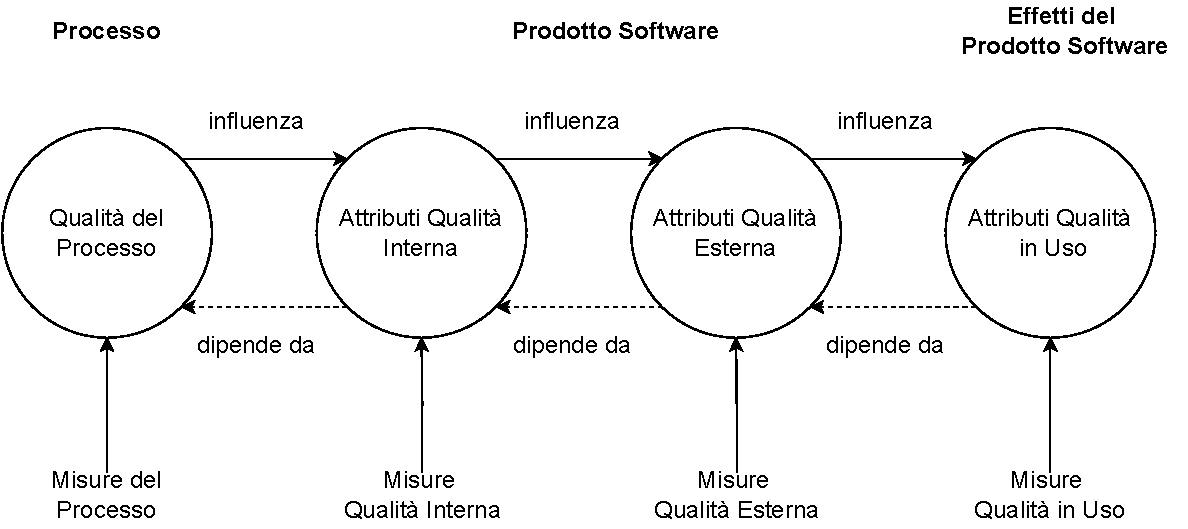
\includegraphics[width=\textwidth]{Figure/Background/quality_cycle_process.pdf}
    \caption{Ciclo di sviluppo della qualità del prodotto software}
    \label{fig:quality_cycle_9126}
\end{figure}

\begin{table}[h!]
\centering
    \begin{tabular}{|c|p{6cm}|}
        \hline
        \textbf{Caratteristiche} & \textbf{Attributi}\\
        \hline
        Funzionalità (Functionality) & Completezza, Accuratezza, Interoperabilità, Sicurezza, Aderenza alla funzionalità. \\
        \hline
        Affidabilità (Reliability) & Maturità, Tolleranza ai guasti, Recuperabilità, Aderenza all'affidabilità.\\
        \hline
        Usabilità (Usability) & Comprensibilità, Apprendibilità, Operabilità, Attrattività, Aderenza all'usabilità. \\
        \hline
        Efficienza (Efficiency) & Comportamento sul tempo di esecuzione, Utilizzo delle risorse, Aderenza all'efficienza. \\
        \hline
        Manutenibilità (Maintainability) & Analizzabilità, Modificabilità, Stabilità, Provabilità, Aderenza alla manutenibilità.\\
        \hline
        Portabilità (Portability) & Adattabilità, Installabilità, Coesistenza, Sostituibilità, Aderenza alla portabilità.\\
        \hline
        Qualità in uso (Quality in use) & Efficacia, Produttività, Sicurezza, Soddisfazione.\\
        \hline
    \end{tabular}
    \caption{Modello di qualità ISO/IEC 9126}
    \label{tab:iso_iec9126}
\end{table}


\section{Technical Debt}
%inizia dicendo che causano problemi alla qualità, parli di technical debt e alcuni lavori che incitano l'importanza di technical debt, 
Come è fondamentale effettuare analisi e monitorare la qualità del proprio prodotto, è altrettanto fondamentale percepire e identificare problematiche che possano danneggiare la qualità.
%%forse una frase che connette ci vuole
Molte industrie e diversi professionisti del software, al fine di poter andare incontro al \textit{time-to-market} (\ie l'ammontare di tempo richiesto per cui un prodotto, a partire dalla concezione dell'idea, raggiunge la fase di distribuzione nel mercato) e altri fattori di business, si ritrovano ad affrontare quello che viene definito come \textit{technical debt}.
La prima definizione di Technical Debt è stata coniata da Ward Cunningham \cite{Cunningham1992td}, dove viene definito come un insieme di scelte di design subottimali o soluzioni implementative che possono influenzare negativamente i dati e la qualità del codice.
Questa iniziale definizione porta al collegamento metaforico del debito finanziario, dove un professionista del software che sceglie di adoperare scelte di design non ottimali può essere associato a una persona che incorre in un debito di pagamento. Quando una persona non salda in tempi regolari e ammissibili il debito assegnato riscontra una forma di interesse. Questa forma di interesse continua a crescere in maniera proporzionale al tempo necessario per poter saldare il debito definito.
Allo stesso modo, quando uno sviluppatore decide di non ripagare il debito creato all'interno del sistema (\ie migliorare la soluzione subottimale introdotta), l'interesse si accumula e l'ammontare del technical debt aumenta. Quindi il costo di mitigazione del technical debt del sistema cresce in modo proporzionale al tempo che intercorre tra l'introduzione del technical debt e la sua mitigazione.
In casi estremi, l'interesse viene accumulato a tal punto da essere impossibile da mitigare, causando danni ingenti al sistema e l'abbandono del prodotto.
Questa particolare casistica viene definita come \textit{technical bankruptcy}. \cite{refactoringSmellSuryanarayana}

La metafora finanziaria del technical debt inoltre ha portato all'adozione della sua terminologia dalla parte dei professionisti di ingegneria del software.
Ampatzoglou et al. \cite{AMPATZOGLOU201552} hanno analizzato la terminologia maggiormente utilizzata per la rappresentazione e l'analisi del Technical Debt nei sistemi e in particolare hanno estratto le definizioni di technical debt \textit{principal} e \textit{interest}:
\begin{itemize}
    \item \textbf{Principal}: ha lo scopo di valutare l'effort richiesto per indirizzare il sistema attuale in un sistema che abbia un livello ottimale di qualità di progettazione. 
    \item \textbf{Interest}: ha lo scopo di valutare l'effort addizionale necessario per applicare tecniche di manutenzione e recuperare la qualità del software.
\end{itemize}
%aggiungi qualcosa per chiudere il discorso perchè sono importanti queste metriche?




Esistono diverse tipologie di technical debt, il quale ognuno è relativo a una specifica granularità del sistema:
\begin{itemize}
    \item \textbf{Code Debt}: conseguenza dell'introduzione di scelte implementative subottimali, come violazioni rilevate da un tool di analisi statica, o uno stile del codice inconsistente.
    \item \textbf{Design Debt}: conseguenza dell'introduzione di design smells e violazione di regole di progettazione.
    \item \textbf{Test Debt}: conseguenza della mancanza gestione delle operazioni di testing o dalla inadeguatezza del raggiungimento dei criteri di testing.
    \item \textbf{Documentation Debt}: conseguenza della mancanza di documentazione o di una scarsa definizione dei dettagli del sistema.
\end{itemize}

In questo lavoro di tesi saranno discusse le istanze di technical debt inerenti all'investigazione effettuata.
Nella prossima sezione quindi sono introdotte le istanze di Technical debt relative al codice del sistema.
\subsection{Code Debt}
\label{sec:code_debt}
L'implementazione del codice sorgente prevede molte decisioni riguardanti lo stile e il design della soluzione. Il codice sorgente può essere soggetto a revisione, ispezione e analisi statica per rilevare i problemi di piccola granularità. Tipici esempi di problemi di implementazione del codice sono la violazioni di standard del codice, una errata nomenclatura, codice duplicato e fuorvianti o incorretti commenti del codice.
Molti di questi sintomi sono definiti come \textit{code smells}. Quando il sistema incorre in technical debt con una granularità al livello del codice, il debito tende a diminuire attributi di qualità come la maintainability a tal punto da rendere difficile di fare le correzioni al sistema quando ne ha bisogno.
I code smell sono definiti come scelte implementative di bassa qualità che possono nascondere problemi più gravi alla qualità del sistema \cite{FowlerCodeSmell}.
Ogni code smell può influenzare diversi aspetti di qualità del codice e possono avere una diversa severità al variare dei possibili danni che possono causare al sistema.
Di seguito saranno elencati e illustrati i code smell più identificati nei sistemi software presenti nello stato della pratica, come riportati da uno studio sulla percezione della presenza e la frequenza dei professionisti del software condotto da Palomba et al \cite{PalombaCodeSmells}.
\subsubsection{God Class}
Un'istanza di \textit{God Class} rappresenta una classe che risponde all'esigenza di multiple responsabilità e contiene quindi un numero alto di funzionalità.
Le problematiche di questa classe non sono causate direttamente dalla sua dimensione, ma da fattori che vanno implicitamente a incidere sulla manutenibilità del software. In particolare, quando viene identificata una istanza di questo genere all'interno del proprio sistema, i seguenti attributi di qualità del sistema hanno gravi conseguenze:
\begin{itemize}
    \item \textbf{Coesione}: Grado di correlazione tra le responsabilità e le funzionalità a cui la classe fornisce soluzione. Se la classe ha un'alta coesione, allora le funzionalità all'interno di essa convergono a fornire una soluzione alla stessa responsabilità. Nel caso in cui viene identificata una \textit{God Class}, questa metrica di qualità tende a decrementare data la tua propensione a includere diverse responsabilità.
    \item \textbf{Accoppiamento}: Grado di misurazione della dipendenza della attuale classe con altre componenti del sistema. Se la classe ha un alto accoppiamento, allora la classe presenta un alto numero di dipendenze. Questo comporta alla riduzione di attributi di qualità come la modificabilità del software (appartenente alla caratteristica di manutenibilità del codice), dove ogni attività di manutenzione del software che include questa componente, comporta ad avere un alto impatto su altre componenti.
\end{itemize}


\subsubsection{Complex Class}
Un'istanza di \textit{Complex Class} rappresenta una classe che contiene metodi che riportano un'alta complessità. Anche se, apparentemente un istanza di \textit{God Class} e un istanza di \textit{Complex Class} possono essere simili, diversi sono gli effetti e i danni in termini di qualità che causano al sistema. In questo caso, quando viene identificata una istanza di questo genere, le gravi conseguenze sono riscontrate in termini di complessità del codice.
In particolare, analizzando le metriche di complessità maggiormente utilizzate, è possibile riscontrare i danni che può causare l'introduzione di una \textit{Complex class}.
\begin{itemize}
    \item \textbf{Cyclomatic Complexity}: Metrica del software utilizzata per indicare la complessità di un programma. È una misura quantitativa ricavata dal numero dei cammini linearmente indipendenti che attraversa il codice sorgente del programma \cite{mccabe1976}. La complessità di ogni metodo presente all'interno di una \textit{Complex Class} incide su questa metrica aumentando vertiginosamente il suo valore, la quale incide su attributi di qualità come la manutenibilità e la comprensibilità del software.
\end{itemize}

\subsubsection{Long Method}
Allo stesso modo in cui una \textit{God Class} tende a centralizzare le responsabilità di un sistema, un'istanza di \textit{Long Method} rappresenta un metodo che contiene diverse responsabilità di una classe, incrementando la difficoltà di manutenzione e di comprensibilità. Per poter analizzare una istanza di questo genere, è necessario fare affidamento anche in questo caso alla misurazione di attributi di qualità come coesione e accoppiamento.



\section{Intelligenza Artificiale}
Il termine intelligenza artificiale ha avuto un processo di evoluzione considerevole negli ultimi anni.
Molte definizioni descrivono l'intelligenza artificiale come la capacità di elaboratori o sistemi robotici di poter eseguire operazioni come l'apprendimento o il prendere decisioni in modo analogo alla capacità degli umani \cite{MWDict,CollinsDict}
Quello che rende l'intelligenza artificiale estremamente diffusa nel mondo accademico e industriale è la sua capacità evolutiva, in particolare nell'ultimo decennio, trasformando questa definizione a tal punto da renderla incompleta.
Una definizione che evidenzia maggiormente lo scopo di questa disciplina è stata fornita da John McCarthy \cite{mccarthy2004}, la quale viene definita come:
\begin{quote}
\textit{    La scienza e l'ingegneria di rendere le macchine intelligenti e in particolare i programmi intelligenti. E' correlata a task simili all'utilizzo del computer per la comprensione dell'intelligenza umana, ma l'intelligenza artificiale non deve limitarsi ai metodi che sono osservabili biologicamente.}
    \end{quote}
Sebbene lo scopo di questa disciplina era inizialmente quello di poter permettere alle macchine di imitare la capacità intellettuale degli umani, ora si ritiene che essa possa andare oltre.
L'attuale definizione porta alla definizione di questa disciplina su più livelli \cite{wiki:Artificial_intelligence}:
\begin{itemize}
    \item \textbf{Artificial Narrow Intelligence:} applicazione dell'intelligenza artificiale al fine di avere la capacità di applicare intelligenza in un determinato problema.
    \item \textbf{Artificial General Intelligence:} applicazione dell'intelligenza artificiale al fine di avere la capacità di applicare intelligenza su tutti i problemi su cui un essere umano può applicare.
    \item \textbf{Artificial Super Intelligence: } applicazione dell'intelligenza artificiale al fine di superare le capacità di applicare intelligenza su tutti i problemi rispetto a un essere umano.
\end{itemize}

\subsection{Machine Learning}

Il machine learning è uno dei rami dell'intelligenza artificiale utilizzato dalle industrie. Esso rappresenta l'insieme di tecniche, metodologie e teorie utili a consentire agli elaboratori di poter apprendere utilizzando metodi matematico-computazionali \cite{Michalski1984MachineL}.
Quest'area di ricerca ha l'intento di permettere alle macchine di riconoscere pattern e creare un sistema di decisioni basandosi sui dati.
In particolare può essere definita come l'applicazione di migliorare sull'esecuzione di un task $T$ rispetto alla misura di performance $P$ basandosi sull'esperienza $E$.
Un tipico esempio per la rappresentazione di un sistema di machine learning è quello del filtraggio delle e-mail spam, come raffigurato in Tabella \ref{tab:spam_example}.


\begin{table}[]
    \centering
    \begin{tabular}{|c|p{7cm}|}
        \hline
         Task (T) & Identificare le e-mail che gli utenti non desiderano ricevere.  \\
         \hline
         Performance (P) & Percentuale di e-mail spam che sono filtrate e percentuale di e-mail che sono incorrettamente filtrate.\\
         \hline
         Esperienza (E) & Database di e-mail etichettate come e-mail spam e o non-spam.\\
        \hline
    \end{tabular}
    \caption{Esempio di rappresentazione di un sistema di Machine Learning}
    \label{tab:spam_example}
\end{table}
A seconda della rappresentazione del task $T$ e dell'esperienza $E$ che si ha a disposizione, è possibile utilizzare diverse tecniche di machine learning, classificabili nelle seguenti tipologie \cite{lecun2015deep}:
\begin{itemize}
    \item Apprendimento supervisionato (Supervised Learning): Questa tipologia di tecnica ha l'obiettivo di creare un modello di predizione utilizzando come input i dati costituiti sia da un insieme di attributi, sia da un attributo target. Attraverso la definizione di questi dati, il modello cerca di comprendere il valore dell'attributo obiettivo (target) su nuove osservazioni, non elaborate prima. Per questo tipo di apprendimento esistono due tipologie che si differenziano in base al tipo di predizione che si vuole effetturare sull'attributo target: classificazione e regressione.
    La prima tipologia si basa sul predire la classe di appartenenza tra le diverse istanze di oggetti, la seconda, anche se concettualmente simile alla classificazione, si basa sul predire il valore dell'attributo target su insieme di valori continui.
    \item Apprendimento non supervisionato (Unsupervised Learning): A differenza delle tecniche di apprendimento supervisionato, questa tipologia prevede l'utilizzo di dati non classificati e che appartengono quindi a strutture sconosciute. In particolare, il termine \textit{non supervisionato} deriva dalla caratteristica che i dati non sono etichettati secondo un determinato attributo target. Una tipica applicazione per le tecniche di questa tipologia sono i task di clustering: lo scopo è quello di effettuare un'analisi al fine di identificare nell'insieme di dati dei sottinsieme (detti \textit{cluster}), la quale suddivisione fornisce informazione sul sott'insieme dei dati.
    \item Apprendimento per rinforzo (Reinforcement Learning): Le tecniche di apprendimento per rinforzo prevedono l'estrazione dei dati tramite l'interazione del modello con l'ambiente. Il modello esegue un'azione e riceve un feedback dall'ambiente il quale sarà fonte di informazioni utile alla decisione di quale sarà la prossima azione da eseguire. In questo modo, il modello comprende quali sono le migliori azioni al fine di massimizzare il risultato. In particolare, attraverso la definizione di politiche di premialità e di penalità, il modello indirizza la serie di scelte al fine di ottenere il più alto punteggio.
\end{itemize}


Per la definizione di un modello di machine learning è necessario andare a pianificare il processo di apprendimento, come illustrato in Figura \ref{fig:ml_process}.
Il processo tipicamente utilizzato prevede quindi di partire dall'estrazione dei dati. La scelta dei dati da estrarre dipende dal problema che si affronta e dalla tipologia di tecnica che si utilizza. 
La qualità dell'insieme dei dati viene poi analizzata. In questa fase saranno identificati tutte le problematiche dei dati che possono comportare al degrado della qualità del modello, come la presenza di \textit{missing value} o \textit{outlier} della distribuzione.
Successivamente i dati vengono trasformati e, in particolare, dalla forma grezza iniziale dei dati sarà avviato un processo di \textit{feature engineering}, il quale ci consente di poter estrarre la serie di attributi che aumentano il livello di rappresentazione e dettaglio dei dati.
Alla fine di questa fase, i dati assumeranno una forma strutturata in base al task da elaborare. Nel caso di utilizzo di una tecnica di apprendimento supervisionato, dai dati sarà estratto un insieme di osservazioni dove ognuna è rappresentata dalla descrizione di un insieme di attributi (definite in letteratura come \textit{features}) e da un'attributo target su cui andare a basare il nostro task di classificazione.
Una volta che i dati sono stati strutturati, è possibile andare a selezionare la tecnica di machine learning di cui si ha bisogno, i parametri di configurazione del modello finale, e infine effettuare l'addestramento attraverso l'analisi di una parte dell'insieme dei dati definita come \textit{training set}.
Il risultato della fase precedente quindi sarà un modello capace di poter effettuare elaborazione del task. Quindi, questo modello sarà soggetto a un processo di validazione al fine di poter misurare le sue performance e verificare la qualità del modello.

\begin{figure}[h]
    \centering
    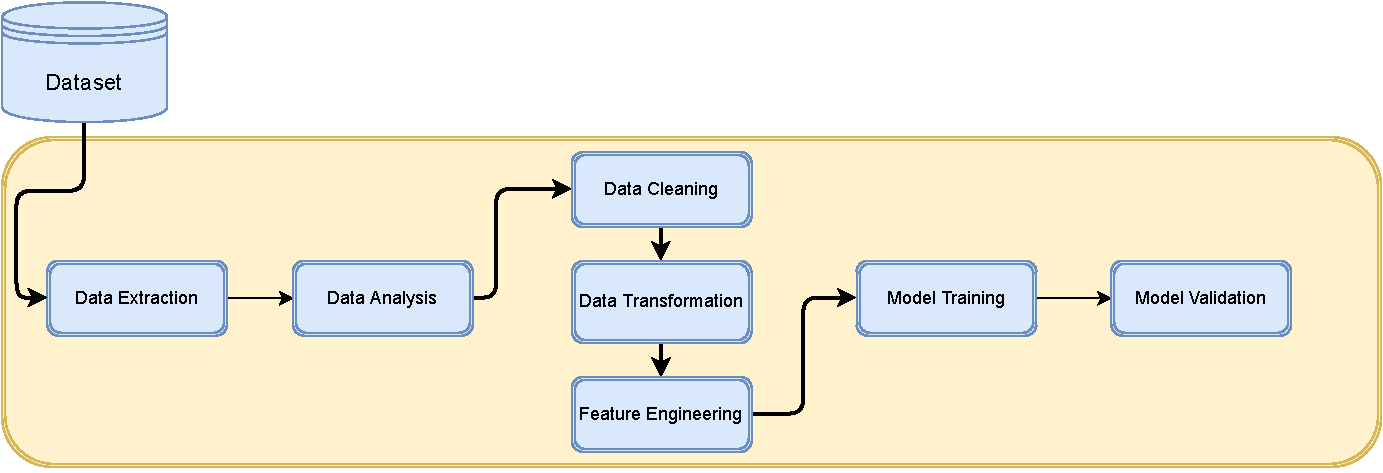
\includegraphics[width=\textwidth]{Figure/Background/ML_Pipeline-2.pdf}
    \caption{Typical Machine Learning process.}
    \label{fig:ml_process}
\end{figure}



\section{Ingegneria del Software per Intelligenza Artificiale (SE4AI)}
\label{sec:se4ai}
L'introduzione di componenti di intelligenza artificiale all'interno dei contesti industriali e del software ha dimostrato un estremo interesse e un'estrema necessità di applicare queste soluzioni al fine di migliorare le pratiche di ingegneria del software.
Tuttavia, al crescere della complessità delle componenti AI nei sistemi software, cresce l'esigenza di poter applicare pratiche di ingegneria del software al fine di poter permettere che queste componenti possano essere manutenute e evolvere nell'ambiente in cui operano.

%Menzies e le 5 leggi dell'SE4AI.
Tim Menzies enuncia quindi le cinque leggi di ingegneria del software per l'intelligenza artificiale al fine di poter divulgare quanto è importante poter creare un'interazione tra queste due discipline \cite{MenziesLaws2020}.
\begin{enumerate}
    \item \textbf{I software AI non comprendono per la maggior parte componenti AI}: Un software AI comprende tantissime componenti che sono da supporto al modello utili a effettuare operazioni come la gestione e l'elaborazione dei dati. Il software può anche includere componenti di business utili a fornire le funzionalità desiderate del sistema. Sculley et al. hanno pubblicato la Figura \ref{fig:sculley_googlesuite}, rappresentando per numero di linee di codice la dimensione delle diverse componenti di un software Google. Evidenziano inoltre che in generale solo una piccola porzione dei sistemi di machine learning è composta da codice machine di machine learning \cite{sculley2015hidden}. E' necessario quindi analizzare e supportare anche la serie di componenti che inglobano il codice AI in un sistema. \\
    \begin{figure}[h]
        \centering
        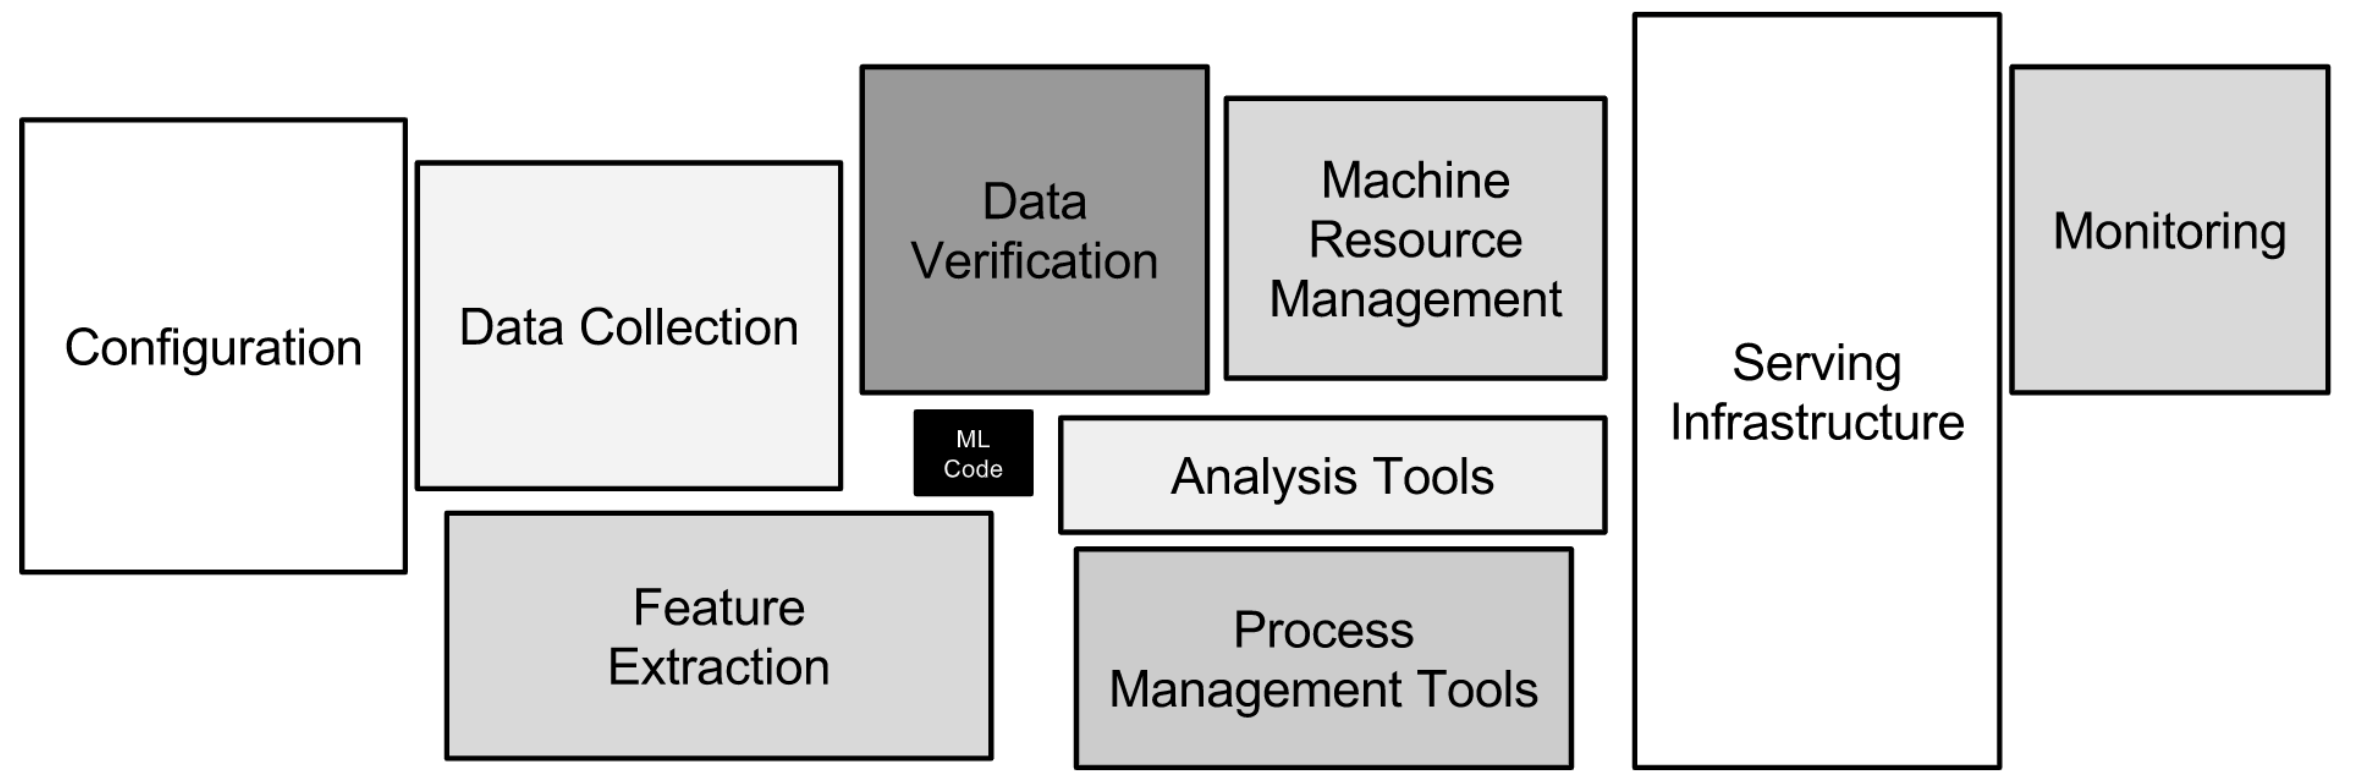
\includegraphics[width=\textwidth]{Figure/Background/sculley-googlesuite.png}
        \caption{Grandezza dei software Google AI in linee di codice, il riquadro nero rappresenta codice \textit{core AI}, i riquadri chiari invece illustrano il codice software di supporto. }
        \label{fig:sculley_googlesuite}
    \end{figure}
    \item \textbf{I software AI hanno bisogno di ingegneri del software}: Tutti i software (AI e non) hanno bisogno di installazione, configurazione, manutenzione e di pratiche che possano trasformare il codice in prodotto.
    Tim Menzies quindi definisce che il futuro dei sistemi software non può essere descritto come l'utilizzo esclusivo di una disciplina. Non può esistere solo ingegneria del software o solo intelligenza artificiale, ma, al contrario, nasceranno promettenti idee dalla combinazione di essi.\\
    \item \textbf{Una cattiva pratica di ingegneria del software implica una cattiva applicazione di AI}: Dal momento che anche l'utilizzo di AI rientra nella creazione di un software, le cattive pratiche di ingegneria del software inficiano anche sul software AI. Sculley riporta in una conferenza che i professionisti di machine learning tendono a utilizzare tutti gli attributi che sono a disposizione dai database aziendali per creare modelli predittivi. Questo comporta all'incremento di technical debt nel modello, in quanto i modelli predittivi costruiti soffrono di una stretta dipendenza con i dati aziendali e, quando sarà effettuato un cambiamento all'interno dei dati aziendali, i modelli predittivi dovranno subire aggiornamenti e manutenzione \cite{SculleyYoutube}. La violazione di principi di qualità del software, come il principio di accoppiamento e coesione, porta conseguenze anche al modello di intelligenza artificiale.
    \item \textbf{Una migliore pratica di ingegneria del software implica una migliore applicazione di AI}: Anche se non è necessariamente vero che applicare metodi di ingegneria del software può migliorare la qualità dell'applicazione AI, diversi professionisti di data science all'interno delle industrie hanno trovato estremi vantaggi nel loro utilizzo. Molti framework, come \textit{scikit-learn} \cite{scikitdoc}, forniscono diverse funzionalità orientate al riuso per avere a disposizione modelli di machine learning e metodi di ingegneria del software (ossia continuos integration, cloud-based testing).
    \item \textbf{Gli ingegneri del software hanno bisogno di particolari tipologie di AI}: Spesso i software di analisi dei dati utilizzano gli algoritmi di AI senza entrare nel dettaglio delle scelte di design del determinato tool. Novielli et al. \cite{NovielliNLP} evidenziano che molti modelli utilizzati nel campo dell'ingegneria del software volti a effettuare \textit{sentiment-analysis} sono costruiti su dati che non sono relativi al dominio d'interesse.
    Questo comporta gravi problemi in termini di performance del modello.
    Quindi, quello che sono considerati tool AI "generali", sono in realtà ristretti all'utilizzo nel dominio in cui sono stati addestrati. Gli ingegneri del software devono utilizzare quindi particolari tipologie di tool AI che siano il più possibile adatte al problema da affrontare.
    
\end{enumerate}

\subsection{Ciclo di vita di un applicazione di machine learning}
Come già definito, le applicazioni di intelligenza artificiale, dato la sua estrema importanza nel campo industriale, si sono evolute in sistemi di larga scala. Questo ha portato un'aumento della complessità di gestione dei determinati sistemi. Uno dei contributi principali che forniscono le pratiche di ingegneria del software alle applicazioni AI è la gestione del ciclo di vita.
Uno dei modelli maggiormente utilizzati è il CRISP-DM (Cross Industry Standard Process for Data Mining) \cite{crispdmWirth}, il quale scopo è di fornire alla comunità scientifica un modello affidabile e efficiente che supporti per ogni fase le applicazioni data-intensive.
Il ciclo di vita è suddiviso quindi in sei fasi, come mostrato in Figura \ref{fig:crisp_dm_process}.
I collegamenti interni del processo identificano le interazioni tra le diverse fasi del progetto e, a seconda dell'output di ogni fase, si decide la successiva fase da eseguire.
I collegamenti esterni esplicitano come il modello ha una natura ciclica. Alla fine dell'esecuzione delle 6 fasi, ovvero successivamente alla fase di deployment del modello, è possibile ricevere dall'ambiente nuovi eventi che scaturiscono la necessità di implementare ulteriori requisiti di business.
\begin{figure}[h]
    \centering
    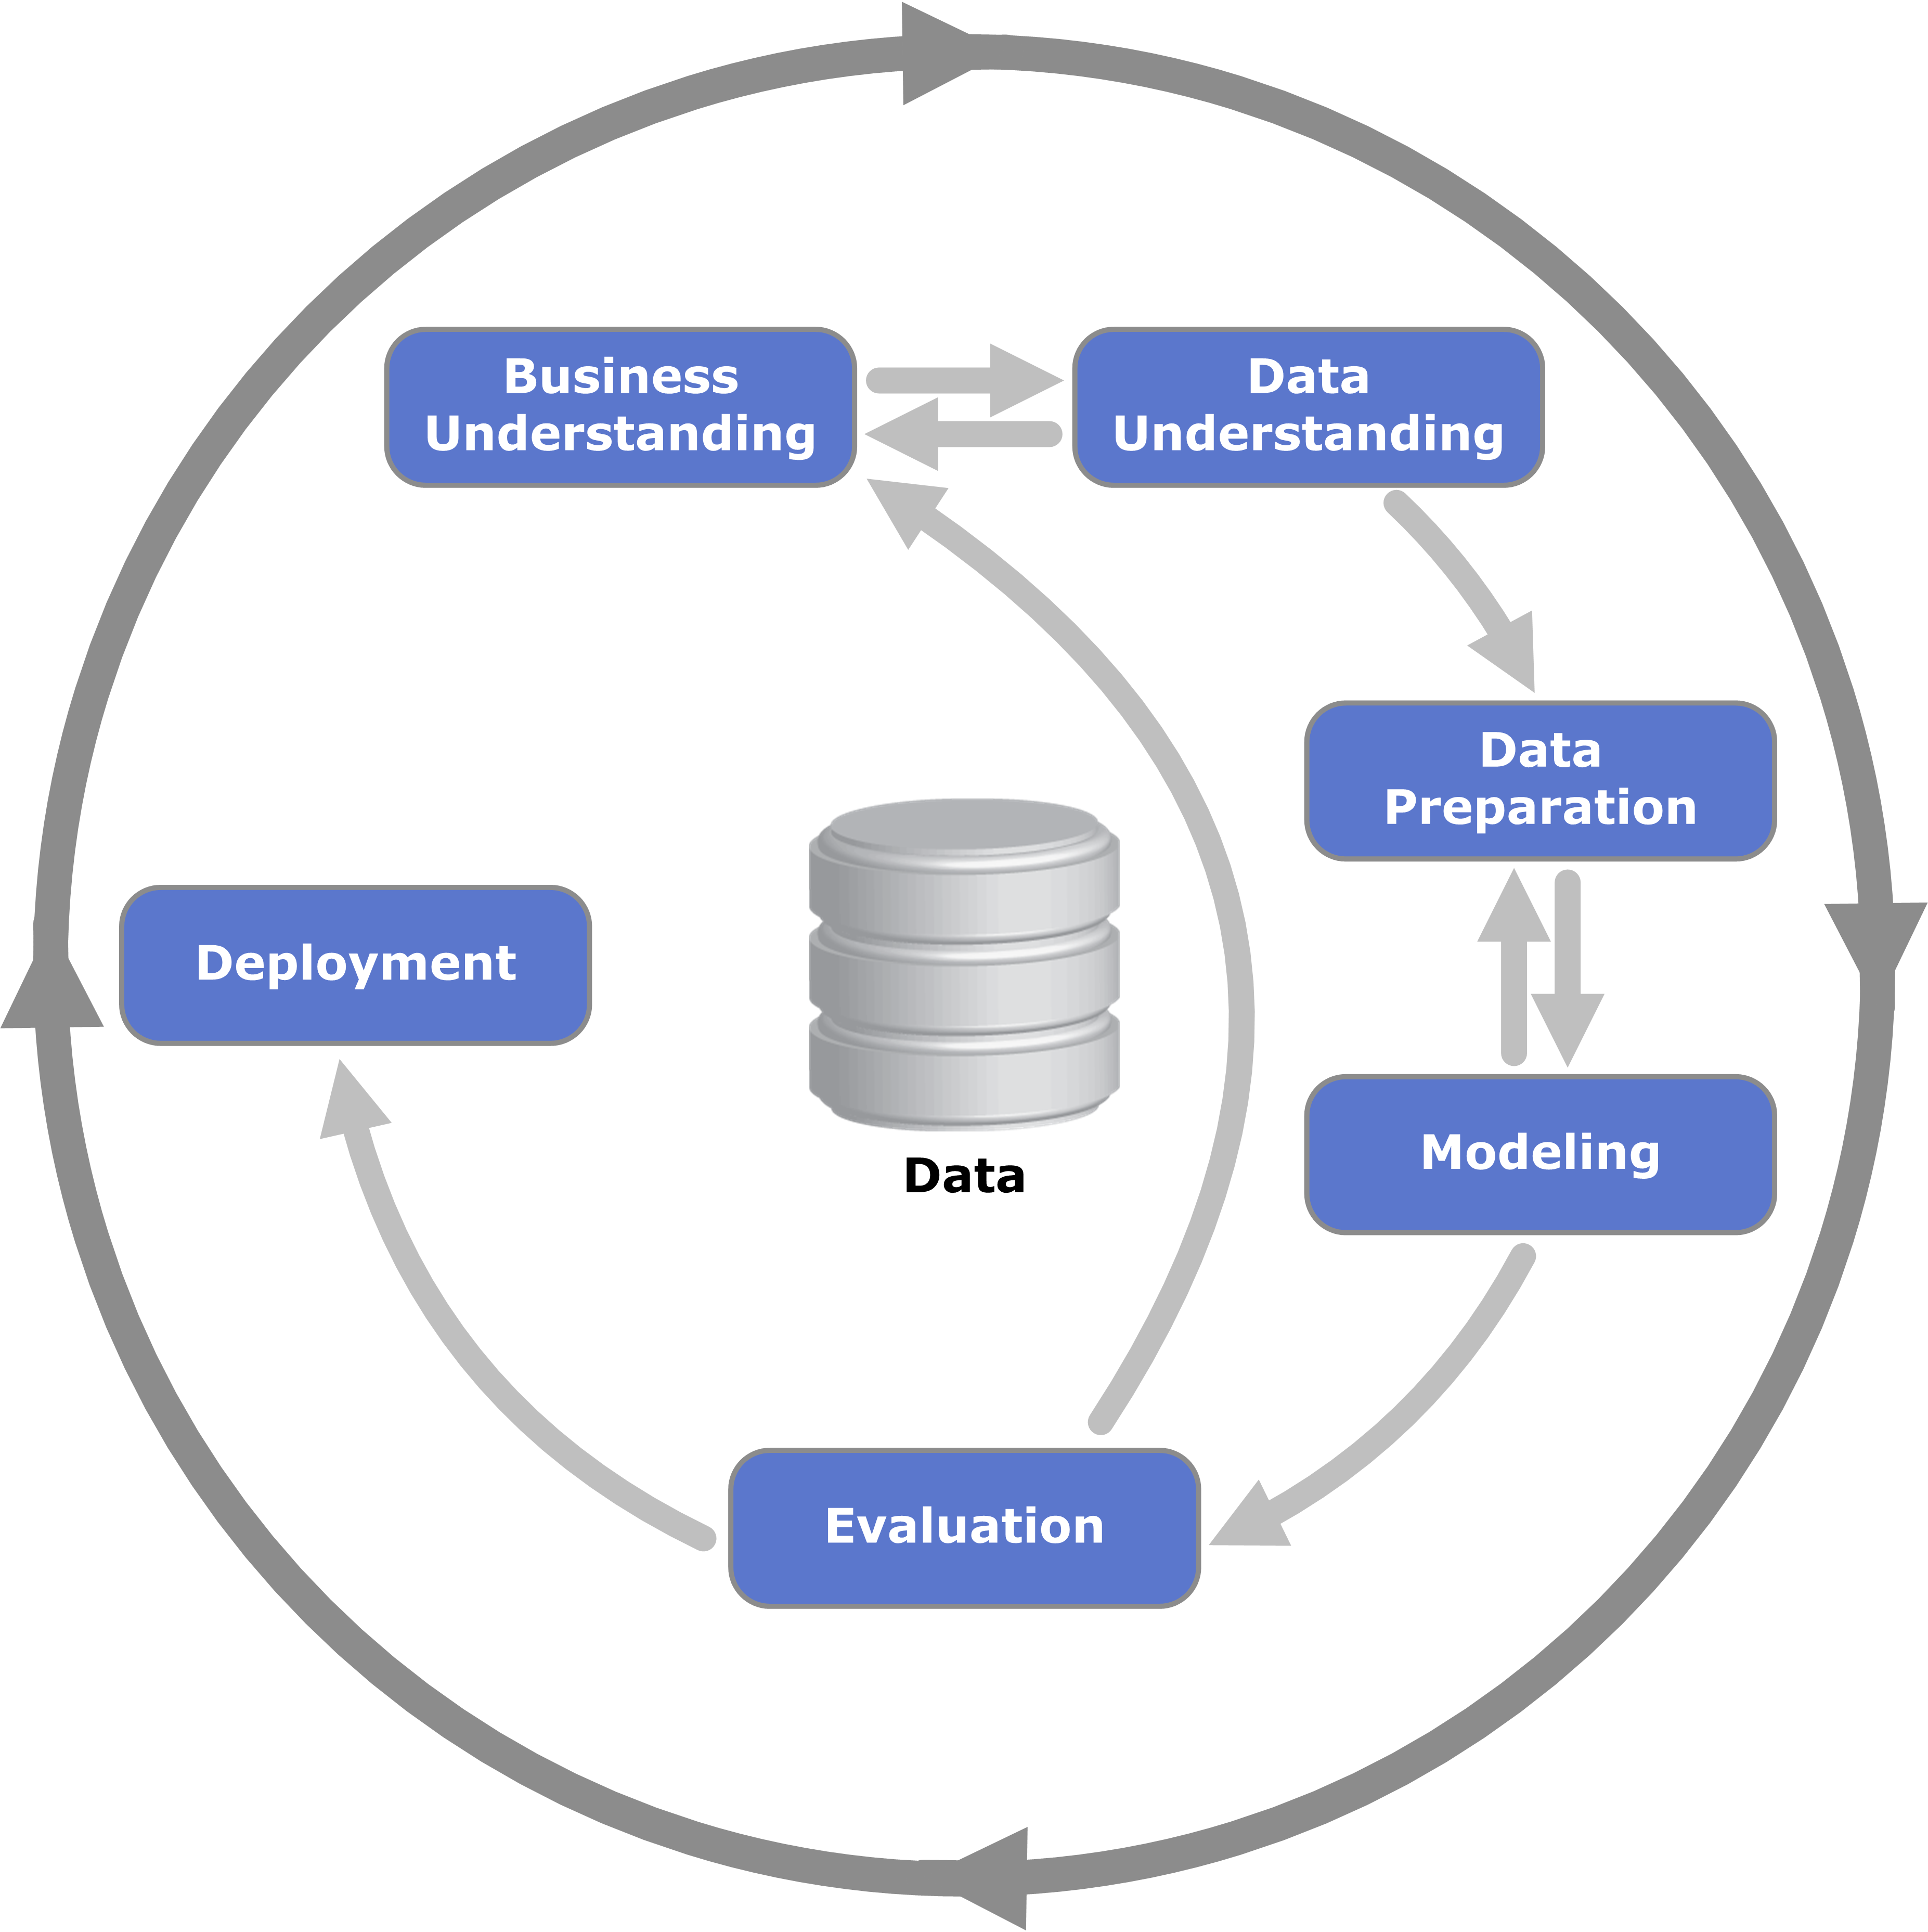
\includegraphics[width=0.5\textwidth]{Figure/Background/CRISP-DM_Process_Diagram.png}
    \caption{Processo di gestione del ciclo di vita CRISP-DM}
    \label{fig:crisp_dm_process}
\end{figure}

Le sei fasi del processo del ciclo di vita CRISP-DM sono definite in:
\begin{itemize}
    \item Business Understanding: Questa fase iniziale ha lo scopo di estrarre gli obiettivi e i requisiti del progetto da un punto di vista commerciale. La conoscenza risultante sarà poi convertita nella definizione di un problema specifico sui dati e infine sarà definita una pianificazione del progetto per raggiungere gli obiettivi.
    \item Data Understanding: Questa fase prevede la collezione dei dati e procede con le attività allo scopo di poter comprendere il dominio su cui si sta procedendo. Saranno quindi identificati problemi di qualità e saranno estratte le informazioni utili al raggiungimento degli obiettivi.
    \item Data Preparation: Questa fase prevede tutte le attività utili alla trasformazioni di un insieme di dati grezzi alla costruzione del dataset finale. Tipiche attività riguardanti la fase di data preparation sono la pulizia dei dati, la selezione degli attributi e la ristrutturazione dei dati.
    \item Modeling: In questa fase diverse tecniche per la creazione di modelli sono selezionate e applicate. Inoltre viene effettuata una configurazione dei parametri del modello al fine di ritrovare i loro valori ottimali e massimizzare le performance del modello.
    \item Evaluation: Una volta che il modello è stato costruito, è importante andare a valutare l'output della fase precedente e revisionare ogni fase del modello, al fine di poter validare che gli obiettivi definiti sono stati raggiunti. Lo scopo è quindi quello di identificare che gli obiettivi di business e i requisiti di qualità siano stati rispettati.
    \item Deployment: L'ultima fase ha come scopo quello di rendere il modello utilizzabile dagli utenti. In questa fase quindi saranno definite la serie di azioni utili a effettuare la distribuzione, l'organizzazione e la presentazione del modello. 
\end{itemize}

%%da aggiungere MLOps


%%%%%%%%%%%%%%%%%%%%%%%%%%%%
\chapter{Stato dell'Arte}


\section{ML-Specific Technical Debt}
I sistemi di Machine Learning hanno una caratteristica predisposizione nell'imbattersi in technical debt, poiché sono presenti ad affrontare sia i tradizionali technical debt di una applicazione, sia gli \textit{ML-Specific technical debt}.
Questa tipologia di technical debt è difficile da rilevare poichè presentano diverse granularità, arrivando quindi a definire la rilevazione anche a livello di sistema.

Sculley et al. \cite{sculley2015hidden} esplicitano il primo approccio alla definizione del \textit{ML-Specific technical debt} a livello di sistema, identificando diverse tipologie di debt che ricoprissero ogni passo della Machine Learning Pipeline:

\begin{itemize}
    \item \textbf{Data dependency debt:} Tipologia di technical debt relativa alla sezione di data management della machine learning pipeline, ovvero considerando le fasi di data ingestion, data collection e data preparation.
    \item \textbf{Analysis debt:} Tipologia di technical debt relativa alla sezione di model management, considerando fasi di feature selection, model selection, model execution e model updating.
    \item \textbf{Configuration debt}: Tipologia di technical debt relativa alla configurazione dei sistemi di machine learning.
\end{itemize}

\subsection{Data Dependency Debt}
Considerando che la data preparation è il primo step per iniziare a costruire un modello di Machine learning, è necessario considerare che il data dependency debt richiede una particolare attenzione per il pericolo che può causare, poichè è possibile che il technical debt impiegato durante la data preparation possa influenzare tutte le successive fasi della machine learning pipeline.
Si definisce quindi il \textit{Data Dependency Debt} quando i dati che si utilizzano all'interno del nostro modello provocano una catena di dipendenze che è difficile da manutenere.
In questa particolare tipologia sono definite tre categorie:
\subsubsection{Unstable Data Dependency}
Il seguente data dependency debt è relativo ai dati o agli \textit{input signals} che sono instabili, ovvero che cambiano il loro comportamento nel tempo.
Tipico esempio di \textit{Unstable Data Dependency} è quando i dati provengono da un altro modello oppure vengono analizzati tramite tecnica di Term Frequency/Inverse Document Frequency (tf/idf) \cite{datamining_rajaraman} il cui score di ogni documento cambia nel tempo.
Questi casi rientrano nel principio \textit{CACE: Changing Anything Changes Everything}, ovvero ogni cambiamento, miglioramento o adattamento all'insieme di dati può portare a un qualsiasi effetto di cambiamento all'interno del modello data la dipendenza dei dati.


\subsubsection{Underutilized Data Dependencies}
Questa tipologia di data dependency debt è relativa alle \textit{feature} degli input o ai \textit{signal} che non portano a incrementi significativi delle performance del modello, avendo come effetto l'aumento dei dati senza significativi vantaggi e la possibilità di introdurre vulnerabilità all'interno del sistema.
Possibili cause che comportano la presenza di \textit{Underutilized Data Dependencies} all'interno del sistema sono:
\begin{itemize}

\item \textbf{Legacy Features:} Si consideri una feature \textit{f} nell'insieme delle feature \textit{S} del modello. Se viene aggiunta una successiva feature \textit{f'} a \textit{S}, è possibile che \textit{f} possa essere ridondante e poco utilizzata dal modello, poichè \textit{f'} contiene la stessa informazione di \textit{f}.

\item \textbf{Bundled Features:} Questa è la situazione in cui al momento dell'aggiunta delle features all'interno del modello, esse vengono valutate nell'insieme, senza considerare una possibile analisi di ogni singola feature. Questa situazione porta che alcune delle features aggiunte non sono causa di un miglioramento delle performance del modello, ma possono risultare in uno scarso guadagno di accuracy.

\item \textbf{Epsilon Features:} Una comune situazione è quella di aggiungere una feature f all'insieme delle feature che permette di avere leggeri miglioramenti alle performance del modello al costo di aumentarne la complessità. 

\item \textbf{Correlated Features:} Si considerino due feature \textit{f} e \textit{f'} inserite all'interno dell'insieme delle feature \textit{S} del modello. Se le due feature hanno un grado di correlazione alto, significa che entrambe le feature trasmettono la stessa informazione, dove solo una delle due è direttamente causale all'altra. I modelli di machine learning hanno problemi a identificare quale delle due feature è da prendere in considerazione.
\end{itemize}

\subsubsection{Correction Cascades}

Questa situazione è ricorrente durante l'aggiornamento e il riutilizzo di un modello. Si consideri un modello \textit{a} per il problema \textit{A}. Questo modello viene riutilizzato per la costruzione di nuovo modello \textit{a'} corrispondente alla soluzione del problema \textit{A'}. Questa correzione, per quanto inizialmente possa apportare vantaggi e utilità alla risoluzione del problema, porta alla costruzione di un modello che dipende per intero da un altro modello. Questa situazione può rincorrere in continui peggioramenti se le correzioni avvengono in cascata, continuando quindi a generare dipendenze tra i modelli.

\subsection{Analysis Debt}
I sistemi di Machine Learning tendono a influenzare il loro stesso comportamento nel tempo. Questo aumenta la difficoltà di predirre il comportamento del sistema prima della sua esecuzione. 
Il fenomeno dove un modello tende a influenzare il suo stesso comportamento durante l'aggiornamento del modello nel tempo viene definito come \textit{Feedback Loop}.
I \textit{Feedback Loops} possono assumere diverse forme, le quali ognuna presenta un alto grado di difficoltà nella identificazione data dovuta dalla loro natura irregolarità della frequenza con cui i modelli si aggiornano.
In particolare sono definite due tipologie di \textit{Feedback Loop}:

\subsubsection{Direct Feedback Loop}
Un modello può direttamente influenzare la selezione dell'ambiente da cui provengono i dati per il training. Se un modello ha un contatto interattivo con l'ambiente da cui percepisce i dati, il proprio output potrebbe essere causa della definizione dei dati. Questo comporta che i dati che il modello successivamente riceve in input per il training del modello in realtà sono dati influenzati.

\subsubsection{Hidden Feedback Loop}
Sebbene le istanze di \textit{Direct Feedback Loop} dispongono di interazioni con l'ambiente visibili e identificabili, diverso è per la presente categoria di Technical Debt.
Un caso più particolare, ovvero la presenza di \textit{Hidden Feedback Loop} nel sistema, riguarda l'interazione indiretta tra due sistemi, i quali si influenzano indirettamente nell'ambiente.

Si consideri un algoritmo di Machine Learning ($\mathbf{M}_{a}$) che ha lo scopo di predirre i luoghi in cui si presenteranno crimini e un altro modello ($\mathbf{M}_{b}$), il quale determina dove distribuire in modo ottimale gli agenti di polizia. 
Il modello $\mathbf{M}_{b}$ distribuisce quindi più agenti di polizia nell'area identificata dal modello $\mathbf{M}_{a}$. Grazie all'incremento del numero di agenti, vengono scoperti più crimini. Il modello $\mathbf{M}_{b}$ riceve informazioni al modello $\mathbf{M}_{a}$, ma influenza anche l'ambiente di input su cui $\mathbf{M}_{a}$ opera per effettuare la predizione. Questa influenza indiretta tra i due modelli risulta in un ciclo continuo di aggiornamento automatico.
Miglioramenti o modifiche a uno dei due modelli di AI porta come effetto un'alterazione del comportamento nell'altro risultando in un possibile degrado delle performance o, in casi peggiori, causando problematiche come l'overfitting.


\subsection{System Level Antipattern}

L'articolo proposto da Sculley et al. \cite{sculley2015hidden} definisce anche due particolari antipattern che sono presenti all'interno delle applicazioni di machine learning, a livello di sistema.


\subsubsection{Glue Code}
I professionisti che contribuiscono alla costruzione di sistemi di Machine Learning e, in particolare, gli esperti di data science tendono a definire soluzioni \textit{general purpose} come singoli \textit{package} indipendenti e autonomi. Quindi, al momento in cui si necessita utilizzare il package in un altro modello o sistema, si tende a inserire ingenti parti di codice che non sono necessarie allo scopo dell'applicazione, ma sono utili ad adattare queste componenti all'interno del sistema.
Un'istanza di \textit{glue code} può portare a lungo termine a un incremento eccessivo dei costi di manutenzione. La continua aggiunta di componenti all'interno di un sistema ha come conseguenza il continuo aumento di risorse necessarie per la gestione dell'applicazione, fi no a giungere al blocco totale del sistema.
Sculley et al. \cite{sculley2015hidden} hanno scoperto che nella comunità accademica solo il 5\% del codice delle applicazioni comprende codice relativo alle operazioni di machine learning, mentre il restante 95\% è rappresentativo di \textit{glue code}.


\subsubsection{Pipeline Jungles}
Questa tipologia di antipattern all'interno del sistema può evolvere ad ogni aggiunta di un dato o una nuova informazione all'interno del sistema.
Questa nuova informazione può richiedere di aggiungere al processo standard definito dalla pipeline ulteriori operazioni per la elaborazione e la preparazione dei dati. Tali aggiunte continue comportano a un incremento della pipeline di machine learning, ritrovandosi in un problema che richiede alti costi di identificazione e di manutenzione.

\subsection{Configuration Debt}
Questa tipologia di technical debt è relativa alla configurazione di sistemi di machine learning.
La gestione e la configurazione dei cambiamenti di un modello, come ad esempio la modifica o l'aggiunta di una \textit{feature}, possono creare situazioni in cui la configurazione diviene difficile da aggiornare.
Tipici esempi che comportano al configuration debt sono:
\begin{itemize}
    \item Una \textit{feature} che, quando utilizzata, richiede per le attività di training il bisogno di utilizzare memoria aggiuntiva al fine di effettuare le operazioni di training del modello in modo efficiente.
    \item Una \textit{feature} che non è più disponibile quindi deve essere sostituita da altre \textit{features} del modello.
    \item Una \textit{feature} che preclude l'utilizzo di altre feature a causa della definizione di vincoli semantici.
\end{itemize}

Gli autori identificano tutte queste caratteristiche come sintomi di una configurazione difficile da modificare e che può causare svariate problematiche al sistema.
Essi propongono quindi una serie di principi di buona pratica per validare il sistema di configurazione utilizzato.
I principi esplicitati dagli autori sono i seguenti:

\begin{itemize}
\item Deve essere semplice specificare una determinata configurazione come un piccolo cambiamento della sua versione precedente.
\item Deve essere difficile commettere errori manuali, omissioni o imprecisioni nella specifica.
\item Deve essere facile visualizzare la differenza di configurazione tra due modelli,
\item Devono essere facilmente verificabili e valutabili i parametri del modello, come il numero di \textit{feature} utilizzate e la chiusura transitiva delle dipendenze dei dati.
\item Deve essere possibile identificare impostazioni ridondanti o inutilizzate.
\item Tutte le configurazioni devono sottostare a un processo di \textit{code review} ed essere validate.
\end{itemize}

\subsection{Common Smells}

Gli autori hanno anche definito una serie di istanze di smells:

\begin{itemize}
    \item Plain-Old-Data Type Smell: I dati sono trasformati in un tipo primitivo come \textit{float} o \textit{integer}. In questa situazione i dati perdono le informazioni relative alla natura del suo formato (detti anche metadati), come l'intervallo di valori ammissibili.
    \item Multiple Language Smell: L'utilizzo di più linguaggi può essere apparentemente una soluzione ottimale che permette l'utilizzo di diverse librerie, ma comporta come effetto collaterale l'aumento dei costi di testing e di comprensibilità delle componenti. La severità di questa particolare istanza di smell aumenta in situazioni in cui la responsabilità della componente viene trasferita ad altri esperti.
    \item Prototype Smell: L'utilizzo di prototipi può essere conveniente per la rappresentazione di idee, ma affidarsi a un ambiente prototipato può portare alla creazione di un sistema instabile e le attività di manutenzione possono conseguire in altissimi costi. 
\end{itemize}

\section{Data Technical Debt}
I sistemi AI sono attualmente considerati data-centric, il quale a differenza dei tradizionali sistemi software, i risultati e la qualità del loro modello dipendono principalmente dai dati piuttosto che il codice \cite{KhomhSE4ML}.
E' necessario quindi comprendere le possibili minacce che possono andare a inficiare la qualità dei dati.
In questo contesto,in uno studio condotto da Foidl et al \cite{FoidlDataSmells}, è stata scoperta la presenza di 36 smells che sono presenti nello stato dell'arte. 
I data smells sono poi categorizzati in base alla loro semantica, sintassi e livello di comprensibilità come segue (Figura \ref{fig:data_smells}):
\begin{itemize}
    \item Believability Smells: relativo alla semantica applicata sui valori dei dati. Questa tipologia di smell indica una bassa "credibilità", dovuta spesso all'utilizzo di valori implausibili. Un esempio di istanza di questa categoria di smell è il \textit{dummy value}, dove viene utilizzato un valore ambiguo per la rappresentazione di un valore mancante. Si consideri ad esempio l'utilizzo del valore "999" per la rappresentazione di un dato mancante. Questo valore può essere facilmente interpretato male a seconda del contesto in cui viene applicato, come nel caso in cui il valore è associato al numero telefonico, esso potrebbe essere interpretato come un numero di emergenza.
    \item Understandability Smells: relativo alla sintassi inappropriata o ambigua dei dati. Questa tipologia di smell può creare problemi di lettura e di elaborazione al software. Un tipo esempio è \textit{l'encoding smell}, in cui un inappropriato tipo assegnato al valore dei dati impedisce di poter fare operazioni su di esso.
    \item Consistency Smells: relativo all'uso inconsistente del formato, del tipo e della rappresentazione dei dati. Un tipico esempio è l'\textit{abbreviation inconsistency} in cui la rappresentazione del valore tramite abbreviazioni o acronimi non è utilizzato in modo consistente in tutti i valori dei dati.
\end{itemize}
\begin{figure}[h]
    \centering
    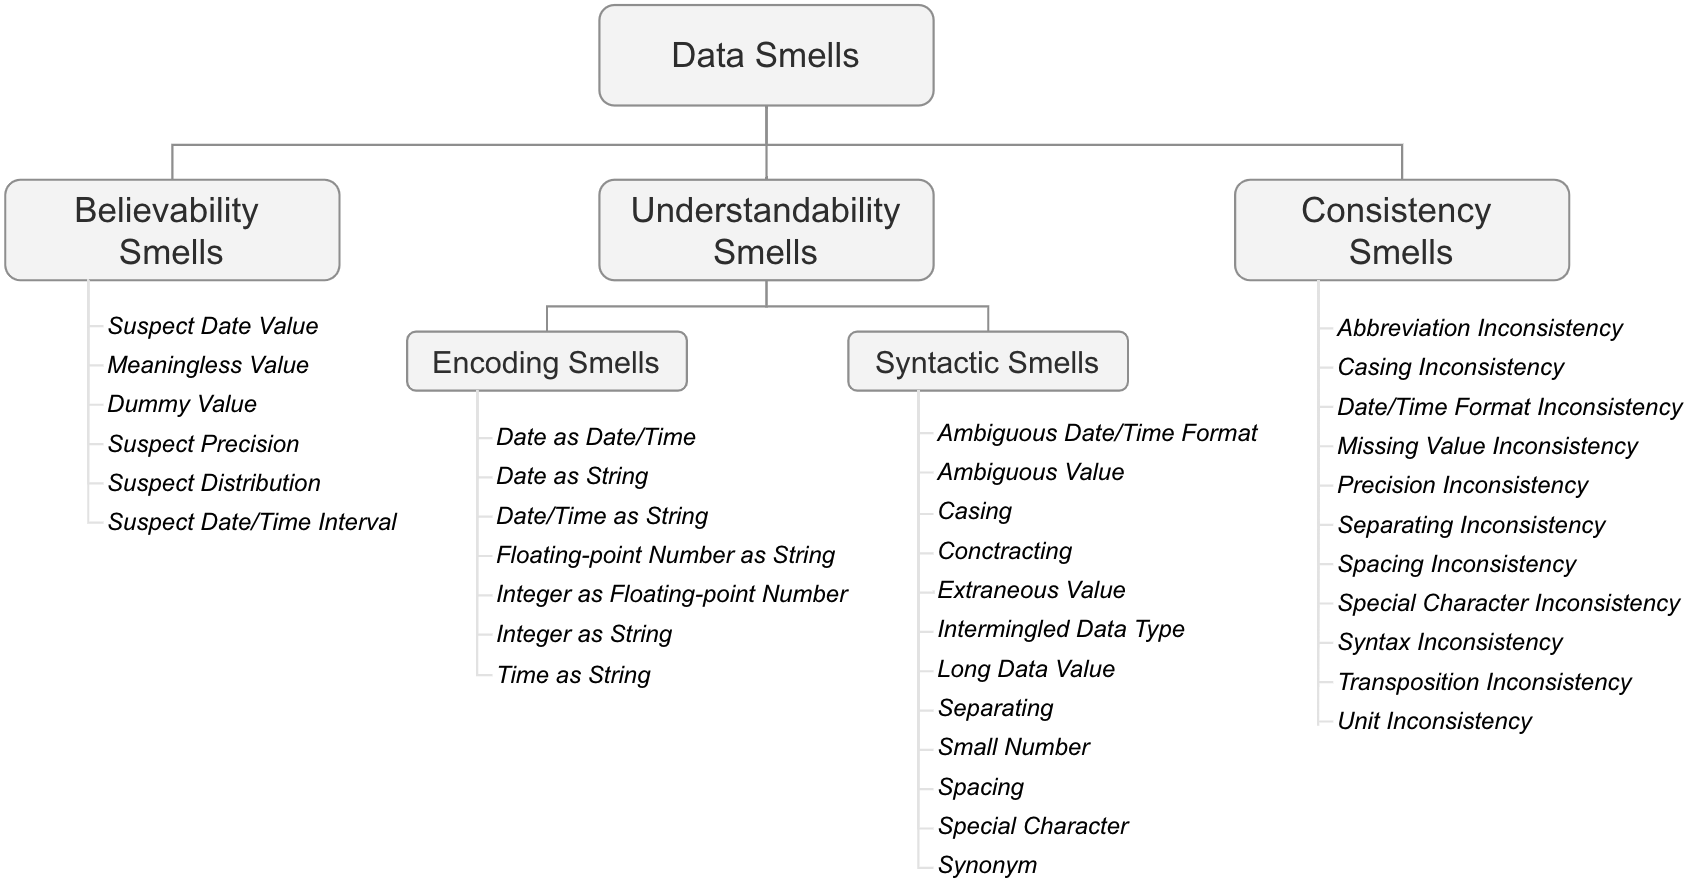
\includegraphics[width=\textwidth]{Figure/StateofArt/data_smell_categories.png}
    \caption{Categorie di Data smells}
    \label{fig:data_smells}
\end{figure}

Inoltre, la rappresentazione inappropriata dei dati non è l'unica minaccia alla qualità del software AI. Secondo uno studio condotto da Sharma et al. \cite{SharmaDBSmells}, anche la violazione di best practice relative alla progettazione di uno schema dei dati può essere causa di introduzione di technical debt nei sistemi. 
Il debito accumulato da una cattiva progettazione dello schema dei dati, come accordato da Al-Barak et al. \cite{Al-BarakDBDebt}, può impattare negativamente non solo sulla qualità, la manutenibilità e l'evoluzione dello schema, ma può inficiare negativamente l'intero sistema.


\section{Code Technical Debt}
I sistemi di intelligenza artificiale sono composti per la maggior parte da codice di supporto alla trasformazione di un modello in un prodotto, come già definito in \ref{sec:se4ai}. Come nei sistemi tradizionali, il technical debt quindi può emergere in questi sistemi per causa dell'introduzione di cattive pratiche del software.
Bogner et al. \cite{bogner2021characterizing} hanno condotto uno studio per analizzare la diffusione dei code smell presenti nei sistemi di intelligenza artificiale. I risultati di questo studio hanno fatto emergere la presenza di \textit{dead experimental code paths} all'interno del codice di produzione. Questa particolare tipologia di smell prevede l'inserimento di sezioni di codice come rami condizionali al fine di poter sperimentare le nuove funzionalità. L'accumulo di codice sperimentale all'interno del sistema di produzione può creare un crescente technical debt che affligge la complessità del sistema e la sua manutenibilità.

Jebnoun et al. \cite{Jebnoun}, attraverso un'analisi comparativa tra progetti di deep learning e progetti tradizionali, hanno riscontrato un'alta frequenza di code smell relativi alla complessità e la lunghezza delle espressioni, arrivando alla conclusione che il codice relativo ai modelli di deep learning includono espressioni più lunghe e più complesse.

Gesi et al. \cite{GesiCSDeepL} hanno inoltre analizzato la diffusione e la severità di code smell all'interno dei sistemi di deep learning in Python, investigando sulla percezione degli sviluppatori. I risultati mostrano un alta frequenza dei seguenti smell:
\begin{itemize}
    \item Scattered Use of ML Libraries: Indica l'utilizzo non sistematico delle librerie di machine learning. All'occorrenza di una modifica sulla determinata libreria, riportare gli aggiornamenti e le modifiche diventa un'operazione onerosa da dover effettuare in diversi punti del sistema.
    \item Unwanted Debugging Code: Indica la presenza di frammenti di codice non più utilizzati all'interno del sistema, aumentando senza alcun beneficio la dimensione e la complessità del sistema.
    \item Deep God File: E' la rappresentazione della God Class nei sistemi di deep learning (come descritta in sezione \ref{sec:code_debt}). Questa componente ingloba diverse funzionalità relative alle fasi del ciclo di vita di un modello di deep learning. 
    \item Jumbled Model Architecture: Le parti dell'architettura del sistema di deep learning sono inglobate aumentando la difficoltà di comprensione e di manutenzione.
\end{itemize}

Queste diverse definizioni della tassonomia di technical debt per sistemi AI permettono di poter analizzare la definizione da diversi punti di vista e con diverse granularità.
Tuttavia, la tassonomia definita dai precedenti autori ha bisogno di maggiori approfondimenti, che permettono di identificare la natura e la causa del technical debt nei sistemi AI.
Naturalmente, essendo le categorie stesse di techincal debt ancora soggette a definizione e raffinamento, è evidente la mancanza di tool automatici a supporto della loro identificazione all'interno di progetti AI-based.
Attualmente, le analisi condotte e presenti nello stato dell'arte prevedono l'applicazione nei sistemi AI della tassonomia dei technical debt presenti nei sistemi tradizionali, senza andare nel dettaglio in possibili istanze che causano technical debt specifiche per l'intelligenza artificiale.
Inoltre molti studi risultano essere complementari al lavoro di tesi, in quanto nello stato dell'arte è presente un maggiore livello di dettaglio su aspetti del sistema di intelligenza artificiale riguardante i dati e il modello. Il presente lavoro di tesi, quindi, contribuisce invece ad aumentare il livello di dettaglio di smell specifici per AI sull'architettura e il codice del sistema, con lo scopo di aggiungere alla tassonomia attuale istanze che sono specifiche e presenti esclusivamente nei sistemi intelligenza artificiale.

%%%%%%%%%%%%%%%%%%%%%%%%%%%%
\chapter{Metodologia}
\chapter{Conclusioni} %\label{1cap:spinta_laterale}
% [titolo ridotto se non ci dovesse stare] {titolo completo}
%

\begin{citazione}
BREVE SPIEGAZIONE CONTENUTO CAPITOLO
\end{citazione}

\newpage


%%%%%%%%%%%%%%%%%%%%%%%%%%%%
\chapter{Analisi e Risultati}
\section{Tassonomia definita in letteratura}
\subsection{Risultati Preliminari}
Lo studio ha riportato dalla collezione per ogni sorgente un'insieme iniziale di 156 articoli, di cui:
\begin{itemize}
    \item 89 articoli provenienti da \textit{Scopus},
    \item 1 articolo proveniente da \textit{IEEEXplore Digital Library},
    \item 21 articoli provenienti da \textit{ACM Digital Library},
    \item 45 articoli provenienti da \textit{Web of Science}.
\end{itemize}
Dalla collezione poi è stata effettuata una rimozione degli articoli duplicati, per giungere a un totale di 80 articoli.
In seguito al processo di revisione manuale di titolo e abstract per ogni articolo tramite l'utilizzo dei criteri di inclusione e di esclusione, 66 articoli sono stati esclusi dai revisori.
In particolare, durante l'analisi preliminare condotta su titolo e abstract dell'articolo, 
9 articoli su 80 sono stati accettati da entrambi i revisori.
Il numero di articoli che hanno ricevuto una valutazione in conflitto sono 8.
I revisori che hanno svolto il ruolo di terzo revisore hanno accettato 5 articoli su 8, avendo come risultato dell'analisi preliminare un totale di 14 articoli.
Inoltre, i risultati del processo di revisione manuale completo hanno portato all'esclusione di altri 8 articoli di ricerca.
Quindi per il primo ciclo di analisi sono stati ritrovati infine 6 articoli di ricerca.
Per estendere i risultati è stato deciso di applicare la tecnica di \textit{backward snowballing} \cite{WohlinSnowballing}.
 Questa tecnica permettere di utilizzare la lista di referenze di ogni articolo per identificare nuovi articoli da includere.
 Il primo passaggio prevede quindi, attraverso l'analisi della lista delle referenze, l'esclusione degli articoli tramite l'utilizzo dei criteri di esclusione.
 Successivamente, si escludono i paper che sono stati già esaminati durante il processo di review. Infine, si riattiva il processo di review per gli articoli che non sono stati esclusi.
 Attraverso l'utilizzo dello snowballing, altri 2 articoli sono stati accettati dal processo di review e inclusi.
 Il processo di revisione della letteratura, quindi, ha come risultato l'estrazione di 8 articoli.
 
 La distribuzione dei paper selezionati sugli anni di pubblicazione è mostrata in Figura \ref{fig:year_chart}.
 Sulla asse delle X è rappresentata la serie degli anni di pubblicazione, mentre sulla asse delle Y è rappresentato il numero di articoli per ogni anno.
 Dal grafico è possibile notare che a partire da una pubblicazione iniziale risalente al 2015, l'interesse da parte dei ricercato è aumentato negli ultimi anni, ritrovando 7 articoli di ricerca pubblicati negli ultimi 4 anni.
 
 \begin{figure}[h]
     \centering
     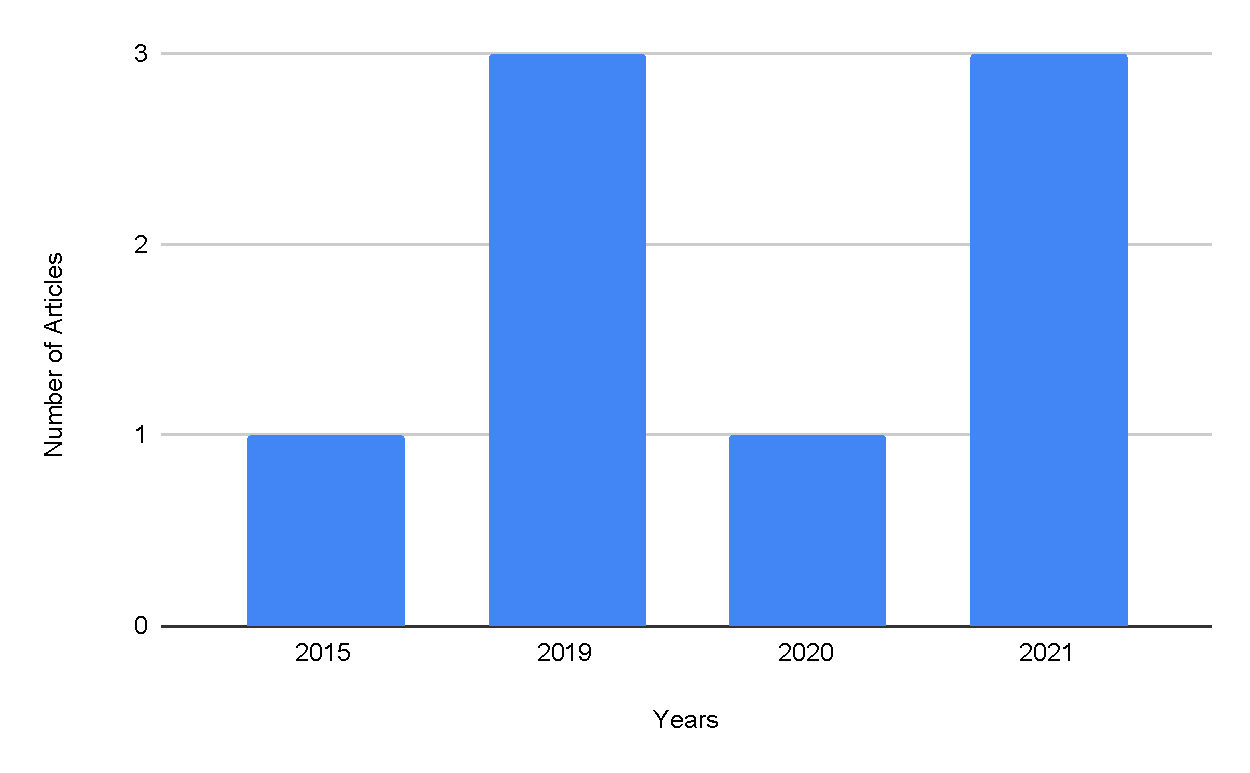
\includegraphics[width=\textwidth]{Figure/Results/SLRResults/year_chart.pdf}
     \caption{Distribuzione degli articoli per anno di pubblicazione}
     \label{fig:year_chart}
 \end{figure}

Tra gli articoli selezionati in questa ricerca ritroviamo 7 articoli che sono che sono stati pubblicati a conferenze internazionali e 1 articolo pubblicato a un workshop. 
In particolare, tra gli articoli pubblicati alle conferenze ritroviamo 1 articolo pubblicato alla "International Conference on Product-Focused Software Process Improvement" (PROFES), 1 articolo pubblicato alla "International Conference on Technical Debt" (TechDebt) e 2 articoli pubblicati alla "International Conference of Software Engineering" (ICSE). 
Questi articoli sono stati pubblicati tutti in conferenze relative all'ingegneria del software, dimostrando quindi che la ricerca relativa all'investigazione di AI Technical Debt ha generato significativo interesse nella comunità di ricerca di ingegneria del software. La lista degli articoli analizzati per questa Systematic Literature review è disponibile nel replication package in \cite{slr_rp}.

\subsection{RQ1.1: Quali tipologie di AITechnical Debt sono presenti in letteratura?}
La Figura \ref{fig:slr_td_type} mostra la distributzione di referenze delle tipologie di AITechnicalDebt nella letteratura.
E' possibile notare come \textit{Data Debt} sia estremamente di riferimento per gli articoli che trattano pratiche di ingegneria del software per i sistemi di intelligenza artificiale, in quanto 5 articoli su 8 trattano questa tipologia di AITechnicalDebt.
Successivamente, con un alto tasso di riferimento, ritroviamo \textit{Configuration Debt}, \textit{Code Debt} e \textit{Architectural Debt}.

\begin{figure}[h!]
    \includegraphics[width=\textwidth]{Figure/Results/SLRResults/RQ1.1/debt_type_count.pdf}
    \caption{Tipologie di AI Technical Debt riscontrate in letteratura}
    \label{fig:slr_td_type}
\end{figure}

In particolare, la Figura \ref{fig:slr_td_instances} mostra la distribuzione di referenze nella letteratura per ogni articolo di ricerca. L'istanza di AI Technical Debt ritrovata maggiormente in letteratura è l'istanza di \textit{Pipeline Jungle}, ritrovando 4 articoli su 8 in letteratura che trattano dei danni che può apportare al sistema AI un incremento smisurato e incontrollato della pipeline AI.
Successivamente, molte istanze di AI Technical Debt sono presenti.
Unstable Data Dependencies, Bundled Features, Correlated Features, Epsilon Features e Feature Entanglement sono le istanze di AI Data Debt che sono state ritrovate, dimostrando l'interesse attuale della ricerca nel trovare metodologie e tecniche utili a preservare la qualità dei dati.

\begin{figure}[h!]
    \includegraphics[width=\textwidth]{Figure/Results/SLRResults/RQ1.1/debt_instance_count.pdf}
    \caption{Istanze di AI Technical Debt riscontrate in letteratura}
    \label{fig:slr_td_instances}
\end{figure}

Analizzando le istanze e le tipologie ritrovate, è possibile conseguire che c'è un'alto interesse della ricerca nell'investire lo sforzo al fine di migliorare le metodologie attuali per preservare la qualità e l'elaborazione dei dati.
Tuttavia, la ricerca ritiene di alto interesse anche gli aspetti architetturali e del codice del sistema AI, riscontrando un alto tasso di interesse rispettivamente per \textit{Pipeline Jungles}, \textit{Glue Code}, e \textit{Multiple Language Smell}.

\subsection{RQ1.2: Quali sono gli approcci di identificazione e mitigazione di AI Technical Debt?}

Sebbene esiste una definizione per le diverse tipologie e istanze di AI Technical Debt, diverso è per le loro tecniche di identificazione e mitigazione.
Possibili spiegazioni estratte dagli articoli in letteratura sono : 
\begin{itemize}
    \item Il codice relativo al modello contiene la minor quantità di codice di tutto il sistema [S01].
    \item I professionisti di data science potenzialmente concentrano i loro al fine di massimizzare le performance del modello, piuttosto che la manutenzione e l'evoluzione del codice AI [S02].
\end{itemize}
Il nostro studio ha riportato come output una singola tecnica di identificazione per la presenza di \textit{Epsilon Feature} all'interno del sistema AI.
La tecnica estratta dalla letteratura è nominata \textit{Leave-One-out Feature Evaluation}.
Si consideri un insieme di feature $F=(f_1,f_2,...,f_n)$ dove con $f_i$ si rappresenta la feature nella struttura dei dati in posizione $i$.
Si estrae e si calcola l'insieme $(F-f_i)$ dove consideriamo l'insieme delle feature rappresentate sottratto da una particolare feature.
Vengono costruiti quindi due modelli $M$ e $M_i$ sui due insieme definiti.
Se la differenza delle performance risultanti dai due modelli non è significativa, significa che il modello $M$ conteneva una particolare istanza di \textit{Epsilon Feature} rappresentata da $f_i$.
Il processo viene poi eseguito ciclicamente per ogni $f_i$ appartenente a $F$.\\


\keyfindingsrqa{
L'interesse della ricerca è focalizzato sullo studio delle istanze di AI Technical Debt relative ai data (data debt), in particolare sulla diffusione e sulla severità di istanze relative alla presenza di dipendenze instabili tra i dati.
Inoltre, un consistente sforzo della ricerca è impuntato verso le istanze di AI Technical Debt incentrate sul codice (code debt), sulla configurazione (configuration debt) e sull'architettura (architectural debt). 
}



\section{Revisione del punto di vista degli sviluppatori}
\subsection{Risultati Preliminari}

Lo studio preliminare è stato condotto su 500 partecipanti.

Il numero di partecipanti che ha risposto correttamente alla domanda filtro è 188, rappresentando il 37,8\% della popolazione, come raffigurato in Figura \ref{fig:pre_filter}.

\begin{figure}[h!]
    \centering
    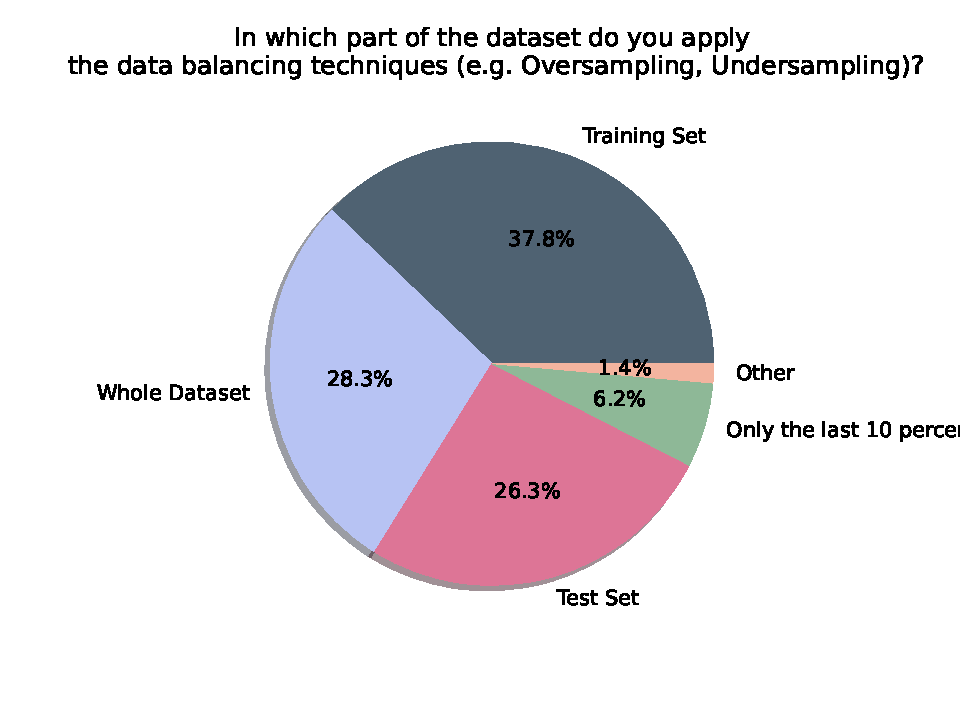
\includegraphics[width=0.8\textwidth]{Figure/Results/SurveyResults/prescreening/prescreening_filter_pie.pdf}
    \caption{Risposte alla domanda filtro del questionario di preselezione}
    \label{fig:pre_filter}
\end{figure}

Infine, applicando i filtri sulle competenze generali del settore e sulle competenze specifiche di intelligenza artificiale, sono stati esclusi 75 partecipanti.
Il numero di partecipanti che è stato accettato per condurre l'esperimento è 113.
La suddivisione dei partecipanti nei tre gruppi sperimentali è stata riportata in Tabella \ref{tab:design_experiment_results}.
\begin{table}[h]
    \centering
    \begin{tabular}{|c|c|c|}
        \hline
        \textbf{Partecipanti} & \textbf{Istanze di Ai Technical Debt}  & \textbf{Numero}\\
        \hline
        Gruppo 1 & Gruppo A+B & 37 \\
        Gruppo 2 & Gruppo B+C & 38\\
        Gruppo 3 & Gruppo A+C & 38\\
        \hline
    \end{tabular}
    \caption{Suddivisione dei partecipanti per gruppi di Ai Technical Debt}
    \label{tab:design_experiment_results}
\end{table}

Tuttavia non tutti i partecipanti hanno deciso di continuare l'esperimento, abbandonando lo studio durante la conduzione dell'esperimento.

Il numero di partecipanti invece a cui è stato sottoposto il questionario finale con successo è 54.

Da ogni risposta sottomessa da ogni partecipante sono state estratte poi i due gruppi sperimentali di riferimento ed è stato possibile quindi ottenere, per ogni gruppo di istanza di AI Technical Debt ottenere il numero di risposte riportato in Tabella \ref{tab:group_exp_results}.


\begin{table}[h]
    \centering
    \begin{tabular}{|c|p{6.5cm}|c|}
    \hline
        \textbf{Gruppi} & \textbf{Istanze AITD} & \textbf{Numero di Risposte}  \\
        \hline
        A &  Glue Code, Multiple Language Smell, Undeclared Consumers & 38 \\
        \hline
        B &  Pipeline Jungles, Correction Cascades, Scattered Use of ML
Libraries & 36 \\
        \hline
        C &  Jumbled Model Architecture, Unwanted Debugging Code,
Deep God File & 34 \\
\hline
    \end{tabular}
    \caption{Numero di risposte per ogni gruppo sperimentale di AI Technical Debt}
    \label{tab:group_exp_results}
\end{table}
%aggiungere la tabella delle risposte con i valori per ogni gruppo.

La Figura \ref{fig:general_skills} e la Figura \ref{fig:ai_skills} mostrano la distribuzione del livello di competenza dei partecipanti su aspetti generali della programmazione, software engineering e intelligenza artificiale, per poi approfondire sulle pratiche di intelligenza artificiale.
In particolare, è possibile notare come i partecipanti in media hanno una discreta conoscenza sulle tre discipline generali definite, riportando nella distribuzione una leggera variazione della mediana, dove le mediane con il valore più alto sono rispettivamente sulla distribuzione delle competenze di programmazione e sulla distribuzione delle competenze di intelligenza artificiale. Questo dato riporta come informazione che il livello di competenza dei partecipanti, anche se leggermente, è maggiormente orientato sulle conoscenze di intelligenza artificiale che quelle di ingegneria del software.
Situazione analoga per le competenze relative alle pratiche di intelligenza artificiale, dove ritroviamo un leggero aumento della mediana a $4/5$ per le attività di data preparation e utilizzo del codice delle librerie di Machine learning.

\begin{figure}[h!]
    \centering
    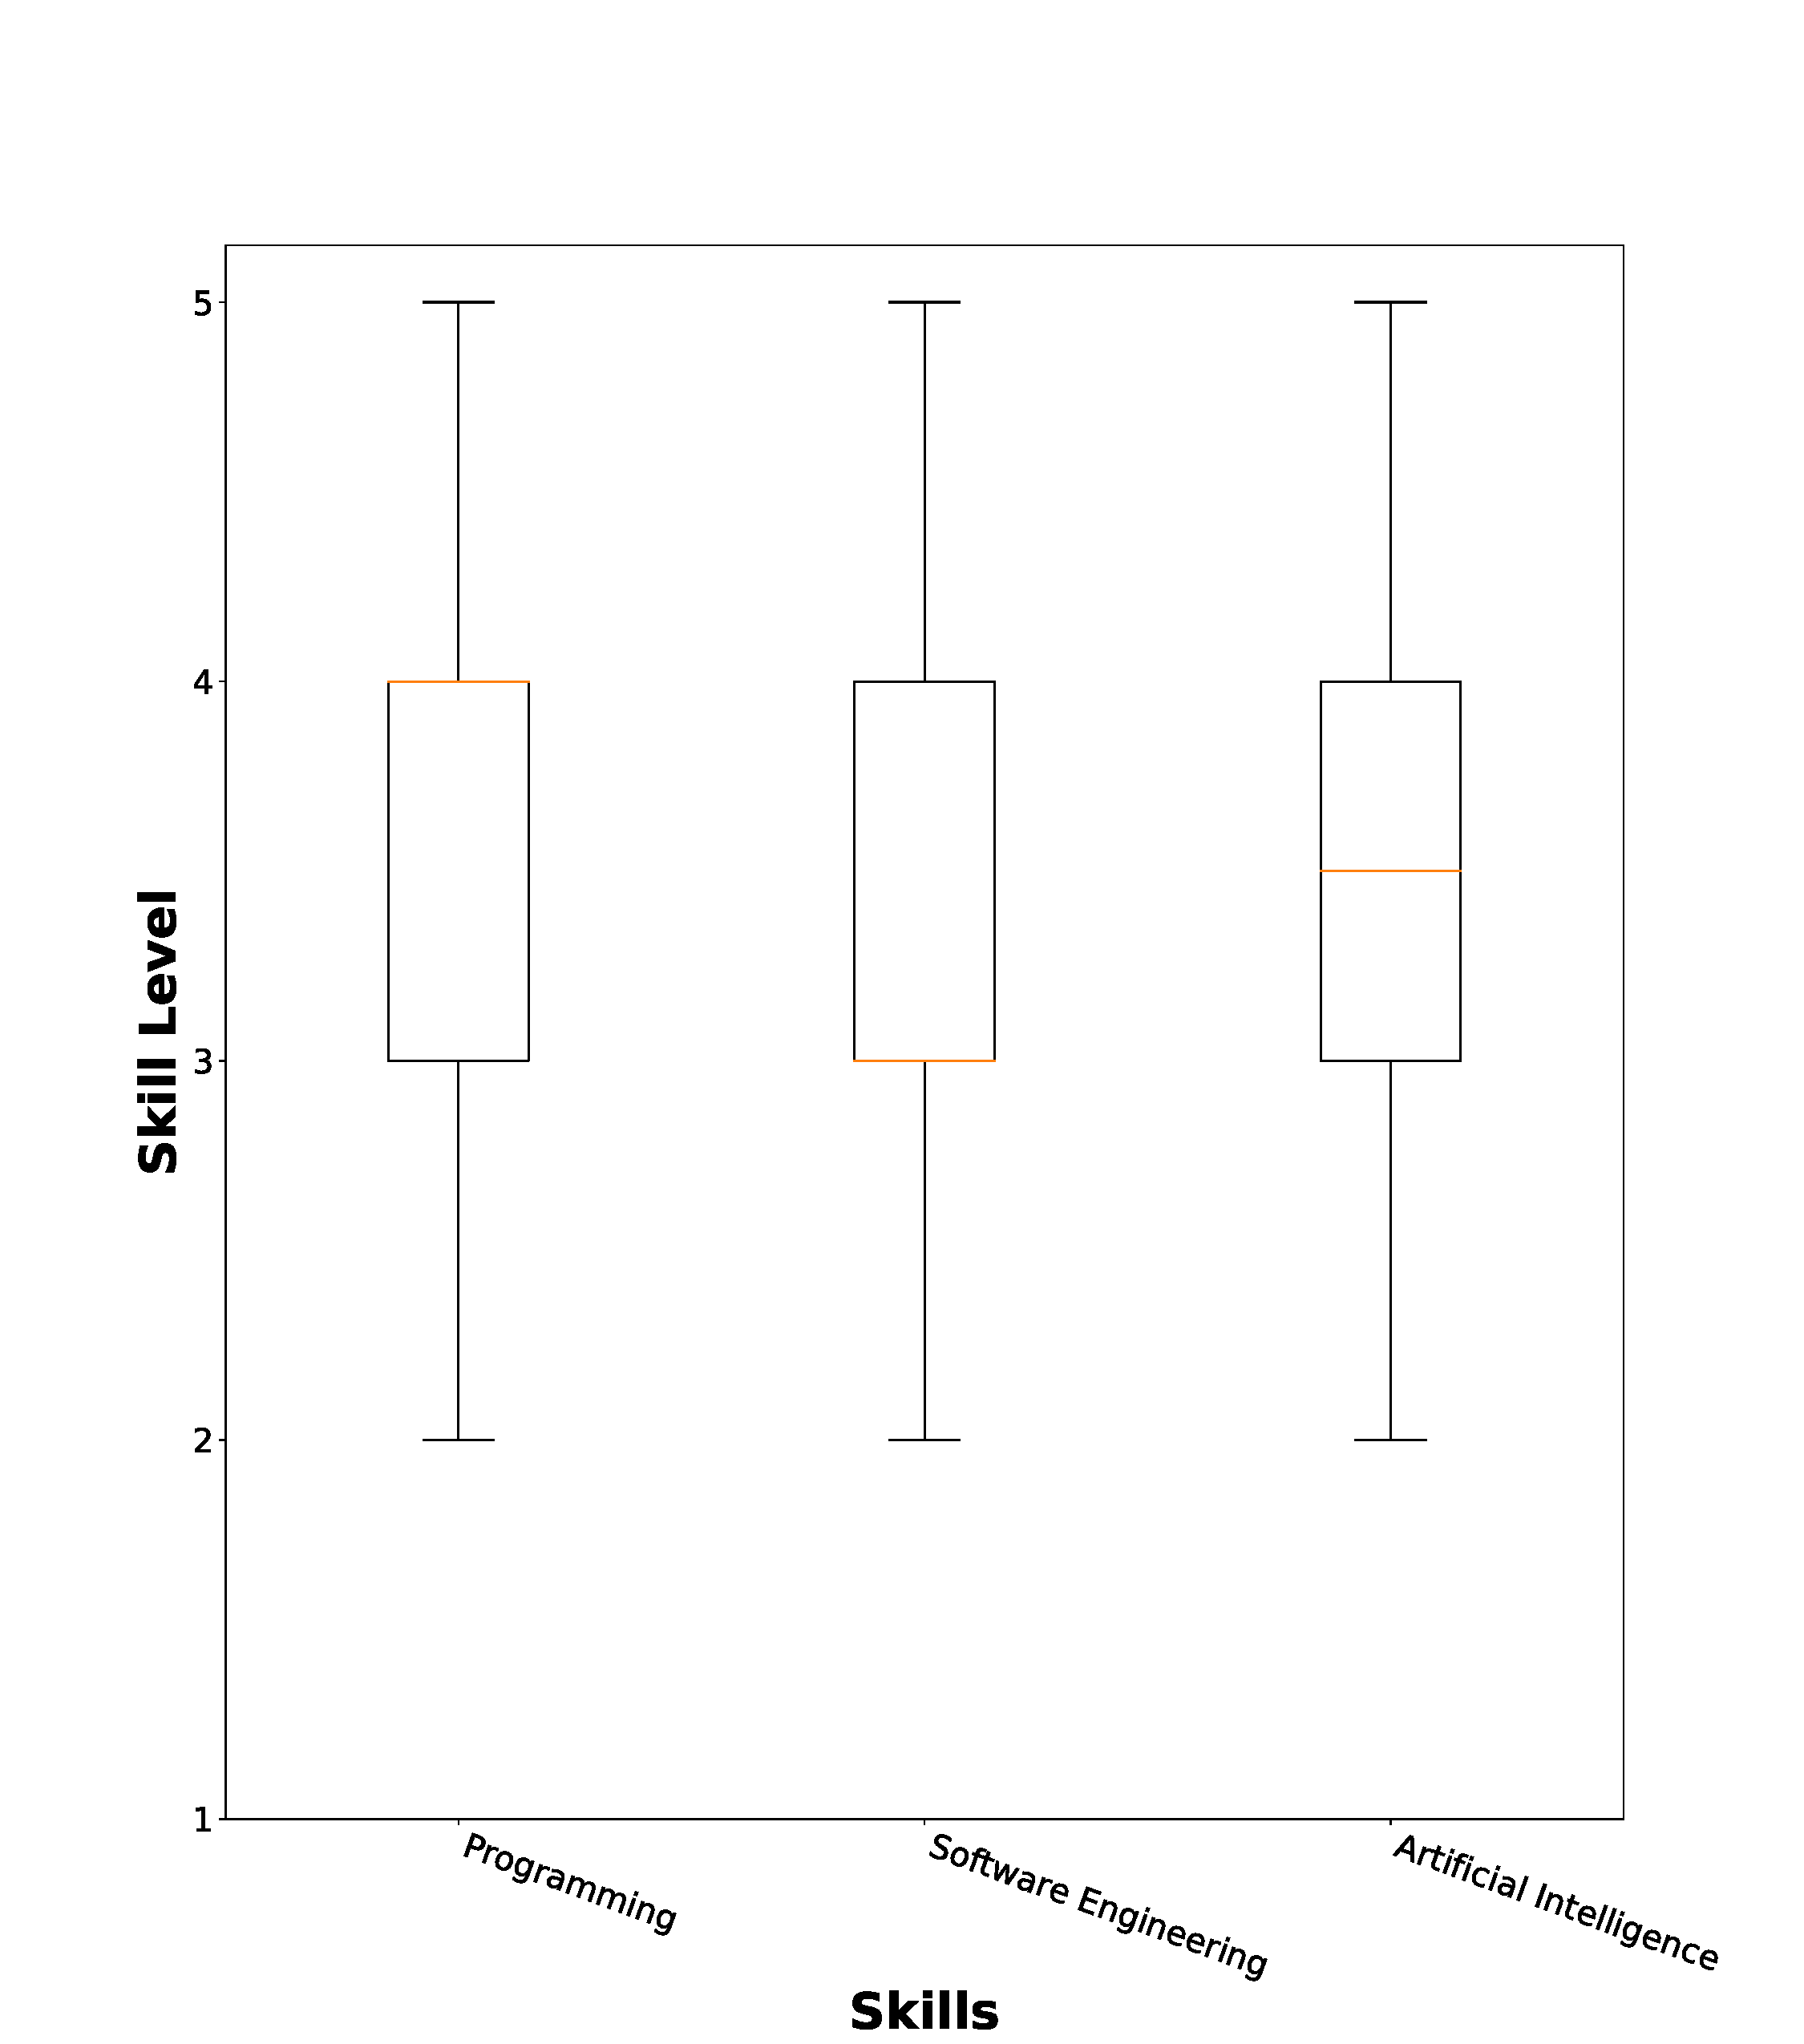
\includegraphics[width=\textwidth]{Figure/Results/SurveyResults/prescreening/def_skills_participant.pdf}
    \caption{Competenze generali dei partecipanti inclusi nel questionario}
    \label{fig:general_skills}
\end{figure}

\begin{figure}[h!]
    \centering
    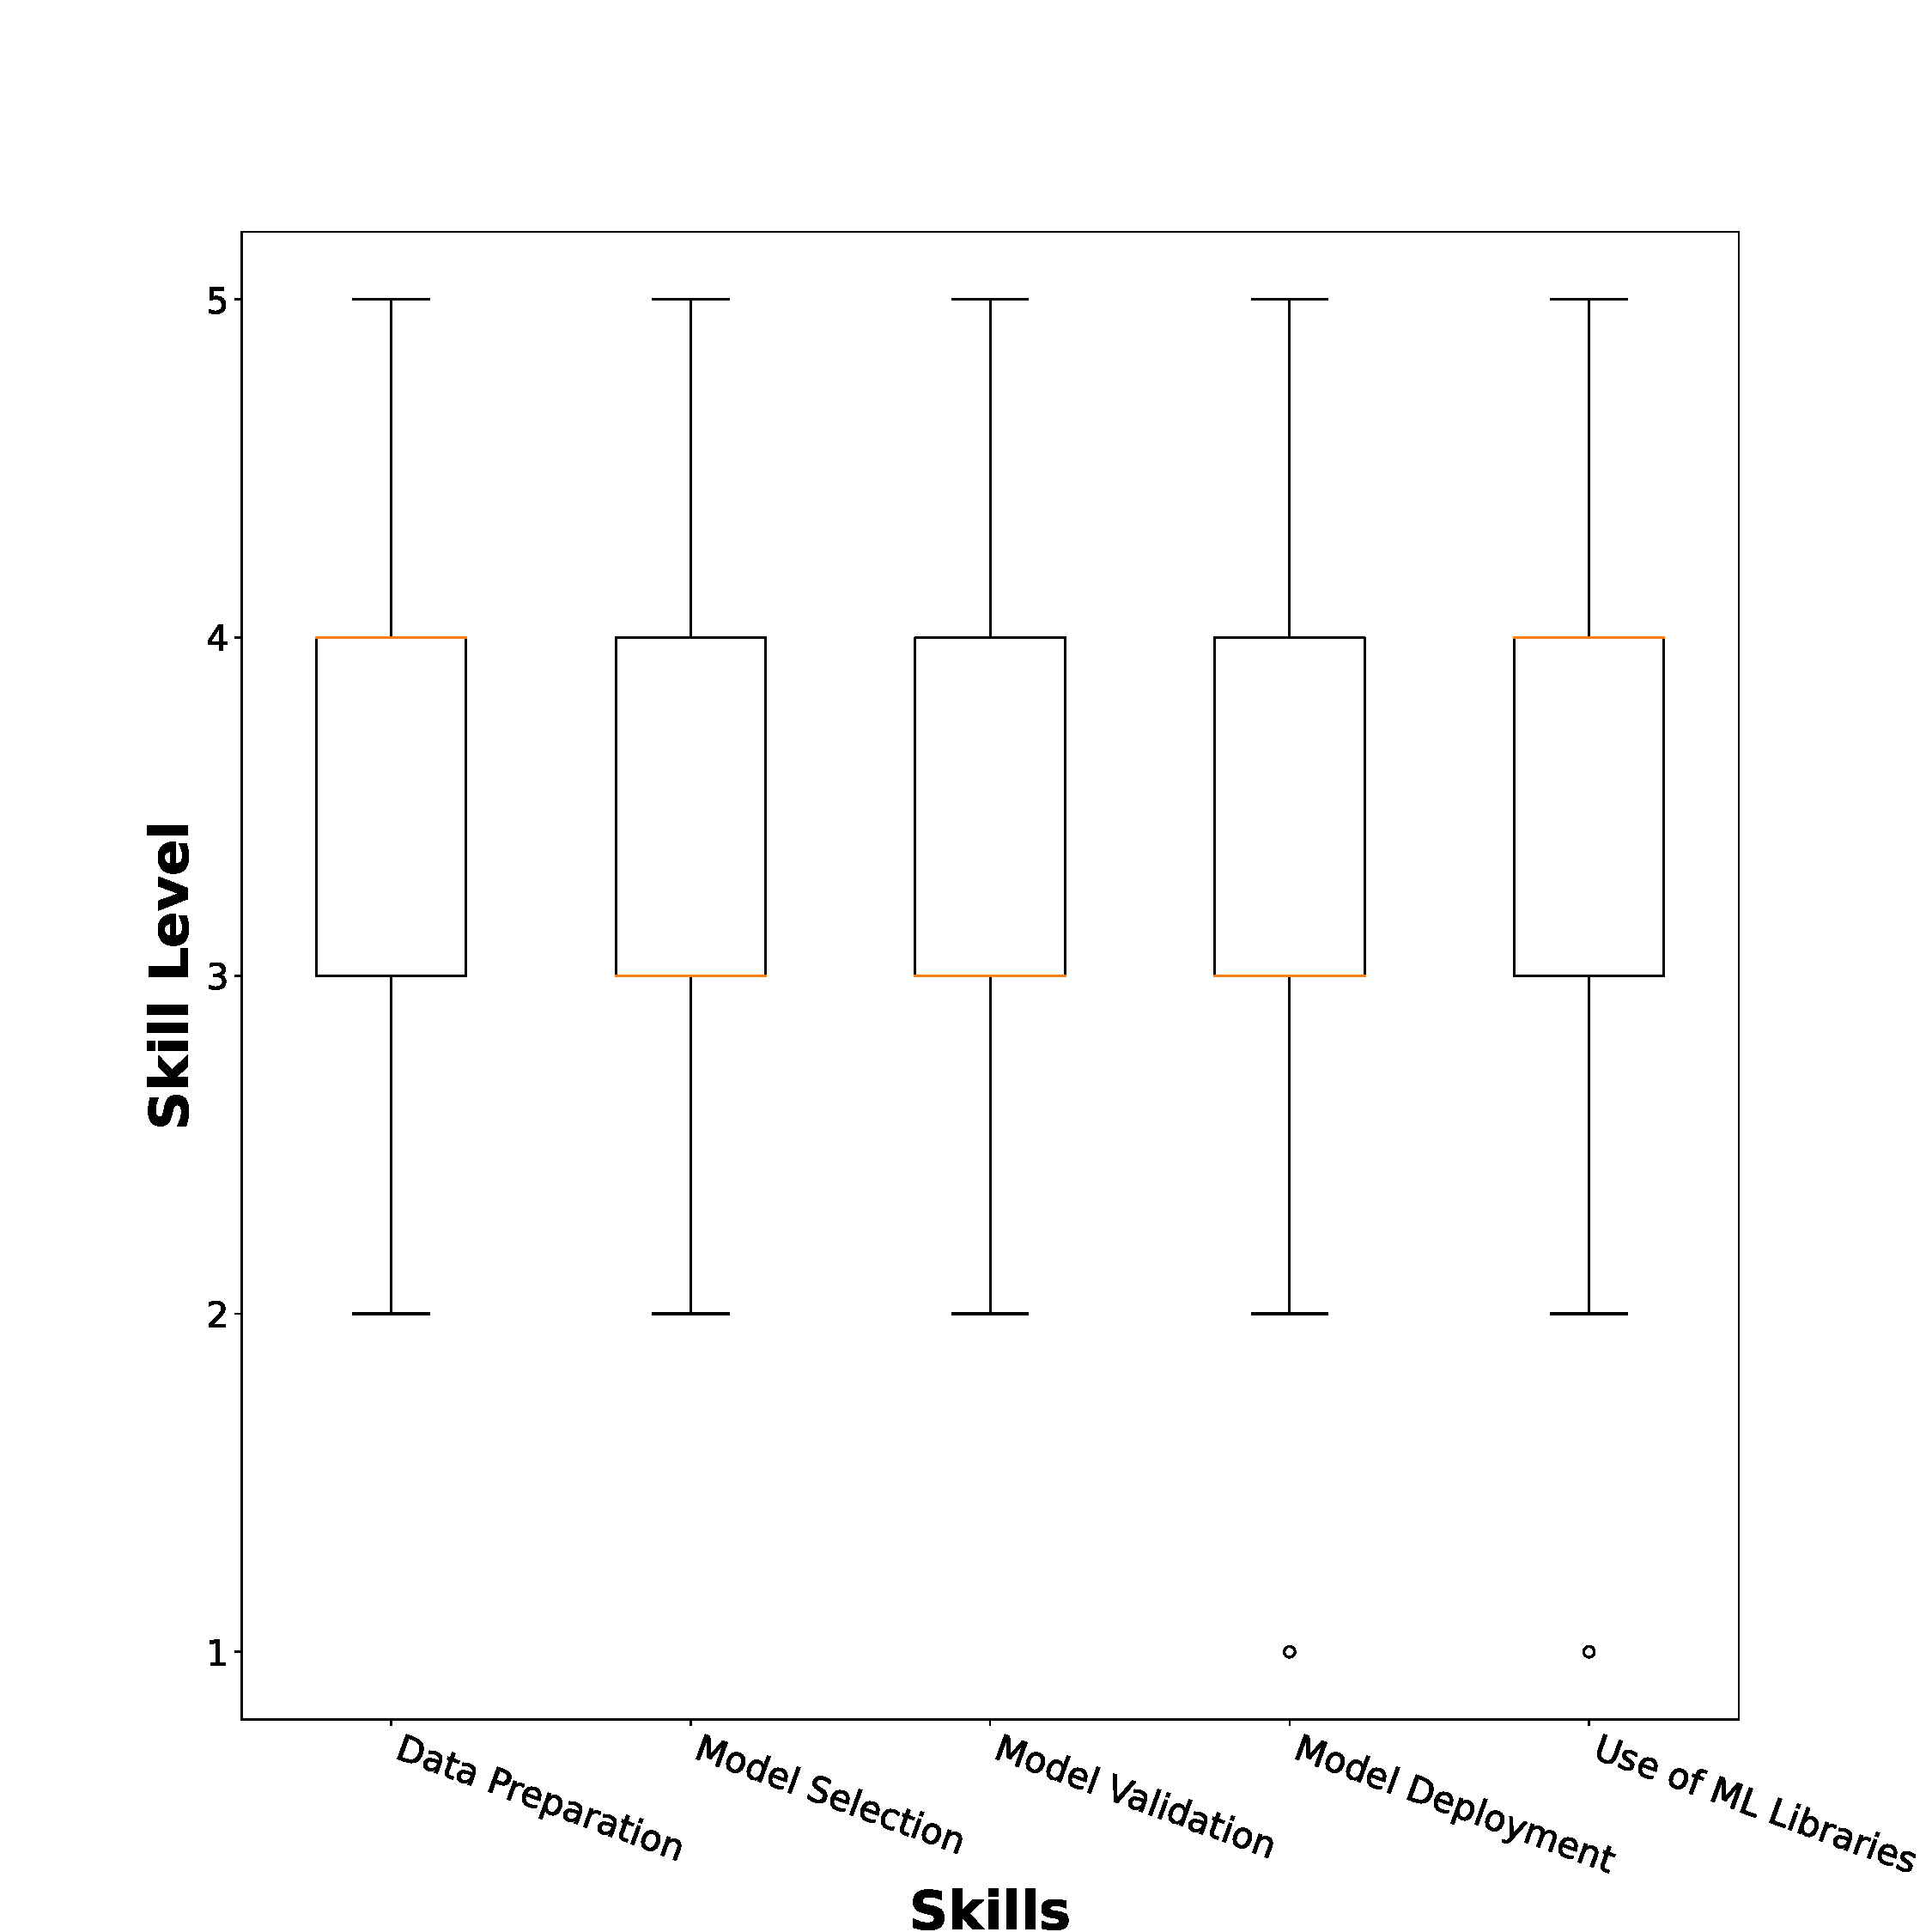
\includegraphics[width=\textwidth]{Figure/Results/SurveyResults/prescreening/def_ai_skills_participant.pdf}
    \caption{Competenze di intelligenza artificiale dei partecipanti inclusi nel questionario}
    \label{fig:ai_skills}
\end{figure}


\subsection{RQ2.1: Quali sono le tipologie di code debt e architectural debt più frequenti secondo la percezione degli sviluppatori AI?}

Secondo le analisi effettuate, i risultati si trovano in accordo con quanto ritrovato nella letteratura.
Considerando gli AI-Technical Debt che sono relativi all'architettura e al codice del sistema, \textit{Pipeline Jungle} e \textit{Glue Code} sono i più diffusi secondo la percezione degli sviluppatori.
La Tabella \ref{tab:freq_index} rappresenta la distribuzione dei valori del livello di frequenza che gli sviluppatori hanno dato per ogni istanza di AI Technical Debt.
In totale, solo 4 particolari istanze di AI Technical Debt vengono percepite da parte degli sviluppatori nel poter avere un'alta frequenza: \textit{Pipeline Jungle}, \textit{Glue Code}, \textit{Jumbled Model Architecture}, \textit{Unwanted Debugging Code}.
Tuttavia, la maggior parte degli sviluppatori ritiene un discreto tasso di frequenza solo per due delle istanze definite:\textit{Pipeline Jungle} e \textit{Glue Code}.

\begin{table}[h]
    \footnotesize
    \centering
    \begin{tabular}{|l|c|c|c|c|}
    \hline
    \textbf{AI Technical Debt Instance} & \textbf{Mediana} & \textbf{Media} & \textbf{Dev. Std.} & \textbf{Moda} \\
    \hline
    Glue Code & \textbf{3.0} & 2.45 & 1.11 & \textbf{3.0} \\
    Multiple Language Smell & 2.0 & 2.05 & 1.11 & 1.0 \\
    Undeclared Consumers & 2.0 & 1.97 & 1.08 & 1.0 \\
    Pipeline Jungle & \textbf{2.5} &\textbf{2.69} & 1.17 & 2.0 \\
    Correction Cascades & 2.0 & 2.44 & 1.03 & 2.0 \\
    Scattered Use of ML Libraries & 2.0 & 2.17 & 1.23 & 1.0 \\
    Jumbled Model Architecture & 2.0 & \textbf{2.53} & 1.02 & 2.0 \\
    Unwanted Debugging Code & 2.0 & 2.5 & 1.24 & 2.0 \\
    Deep God File & 2.0 & 2.18 & 1.03 & 2.0 \\
    \hline
    \end{tabular}
    \caption{Distribuzione della diffusione di AI Technical Debt secondo la percezione degli sviluppatori}
    \label{tab:freq_index}
\end{table}

\subsection{RQ2.2: Quali sono le tipologie di code debt e architectural debt più problematiche secondo la percezione degli sviluppatori AI?}

Gli sviluppatori hanno riportato tre particolari istanze di AI Technical Debt come problematiche all'interno del sistema. 
\textit{Undeclared Consumers}, la quale presenta una moda di severità pari al massimo nella distribuzione dei dati, è considerato per gli sviluppatori il più problematico per i sistemi AI,come illustrato in Tabella \ref{tab:sev_index}.
Le motivazioni raccolte dai partecipanti sono riguardanti l'aspetto di sicurezza, in quanto la presenza di questa particolare istanza di AI Technical Debt può essere sfruttata al fine di comprendere il funzionamento del modello di intelligenza artificiale e effettuare attacchi malevoli.
In particolare, un partecipante ha risposto spiegando che si trova molto spesso a lavorare con dati sensibili e questo può essere una grave falla di sicurezza utilizzabile per diffondere quei dati.
Inoltre la percezione degli sviluppatori ha riscontrato un'alta severità per le istanze di \textit{Pipeline Jungle} e \textit{Jumbled Model Architecture}.
Entrambe le istanze causano una crescita incontrollata del sistema, riportando gravi problematiche di complessità e manutenibilità.
In particolare, un partecipante, in considerazione della presenza di un istanza di \textit{Jumbled Model Architecture} ha risposto che la problematica nasce quando si ha a che fare con un sistema di grandi dimensioni, dove uno sviluppatore in fase di manutenzione del sistema deve affrontare una mancanza di chiarezza e di riconoscibilità delle componenti.

\begin{table}[h]
    \footnotesize
    \centering
    \begin{tabular}{|l|c|c|c|c|}
    \hline
    \textbf{AI Technical Debt Instance} & \textbf{Mediana} & \textbf{Media} & \textbf{Dev. Std.} & \textbf{Moda} \\
    \hline
    Glue Code & 3.0 & 2.92 & 1.32 & 2.0 \\
    Multiple Language Smell & 3.0 & 3.0 & 1.47 & 4.0 \\
    Undeclared Consumers & \textbf{4.0} & \textbf{3.73} & 1.32 & \textbf{5.0} \\
    Pipeline Jungle & \textbf{4.0} & 3.47 & 1.13 & 4.0 \\
    Correction Cascades & 3.0 & 3.22 & 1.22 & 4.0 \\
    Scattered Use of ML Libraries & 3.0 & 3.02 & 1.38 & 4.0 \\
    Jumbled Model Architecture & \textbf{4.0} & 3.47 & 1.0 & 4.0 \\
    Unwanted Debugging Code & 2.0 & 2.32 & 1.22 & 1.0 \\
    Deep God File & 3.0 & 3.11 & 1.45 & 2.0 \\
    \hline
    \end{tabular}
    \caption{Indice di severità delle diverse istanze di AI Technical Debt secondo la percezione degli sviluppatori.}
    \label{tab:sev_index}
\end{table}

In aggiunta lo sforzo di identificazione e lo sforzo di mitigazione delle istanze di AI Technical Debt percepito dagli sviluppatori è riportato rispettivamente in Tabella \ref{tab:id_effort_index} e in Tabella \ref{tab:ref_effort_index}.
Anche sotto questo aspetto, gli sviluppatori ritengono che l'identificazione e la mitigazione per le istanze di \textit{Undeclared Consumers, Pipeline Jungle} e \textit{Jumbled Model Architecture} richiede un'alto effort.
Essendo istanze di AI Technical Debt che interferiscono sul sistema a livello architetturale, queste istanze portano un calo degli attributi di qualità su tutta l'architettura del sistema. Questa granularità così alta, a differenza dei dati e del codice, comporta ad aumentare la difficoltà di identificare e mitigare un problema presente.
Inoltre, in caso di presenza di istanze come \textit{Correction Cascades} o \textit{Deep God File}, gli sviluppatori ritengono che la mitigazione di queste particolari istanze possa richiedere un'alto effort.

\begin{table}[h!]
    \footnotesize
    \centering
    \begin{tabular}{|l|c|c|c|c|}
    \hline
    \textbf{AI Technical Debt Instance} & \textbf{Mediana} & \textbf{Media} & \textbf{Dev. Std.} & \textbf{Moda} \\
    \hline
    Glue Code & 3.0 & 2.92 & 1.32 & 2.0 \\
    Multiple Language Smell & 3.0 & 3.0 & 1.47 & 4.0 \\
    Undeclared Consumers & \textbf{4.0} & \textbf{3.74} & 1.33 & \textbf{5.0} \\
    Pipeline Jungle & \textbf{4.0} & 3.47 & 1.13 & 4.0 \\
    Correction Cascades & 3.0 & 3.22 & 1.22 & 4.0 \\
    Scattered Use of ML Libraries & 3.0 & 3.03 & 1.38 & 4.0 \\
    Jumbled Model Architecture & \textbf{4.0} & 3.47 & 1.02 & 4.0 \\
    Unwanted Debugging Code & 2.0 & 2.32 & 1.22 & 1.0 \\
    Deep God File & 3.0 & 3.12 & 1.45 & 2.0 \\
    \hline
    \end{tabular}
    \caption{Sforzo di identificazione delle diverse istanze di AI Technical Debt secondo la percezione degli sviluppatori.}
    \label{tab:id_effort_index}
\end{table}

\begin{table}[h!]
    \footnotesize
    \centering
    \begin{tabular}{|l|c|c|c|c|}
    \hline
    \textbf{AI Technical Debt Instance} & \textbf{Mediana} & \textbf{Media} & \textbf{Dev. Std.} & \textbf{Moda} \\
    \hline
    Glue Code & 3.0 & 2.95 & 1.23 & 2.0 \\
    Multiple Language Smell & \textbf{4.0} & 3.24 & 1.57 & 4.0 \\
    Undeclared Consumers & \textbf{4.0} & 3.53 & 1.29 & 4.0 \\
    Pipeline Jungle & \textbf{4.0} & 3.33 & 1.17 & 4.0 \\
    Correction Cascades & \textbf{4.0} & 3.5 & 1.18 & 4.0 \\
    Scattered Use of ML Libraries & 3.0 & 3.0 & 1.41 & 2.0 \\
    Jumbled Model Architecture & \textbf{4.0} & \textbf{3.82} & 1.03 & \textbf{5.0} \\
    Unwanted Debugging Code & 2.0 & 2.09 & 1.24 & 1.0 \\
    Deep God File & \textbf{4.0} & 3.71 & 1.19 & 4.0 \\
    \hline
    \end{tabular}
    \caption{Sforzo di mitigazione delle diverse istanze di AI Technical Debt secondo la percezione degli sviluppatori.}
    \label{tab:ref_effort_index}
\end{table}

\subsection{RQ2.3: Qual è l’impatto causato dai code debt e architectural debt secondo la percezione degli sviluppatori AI?}

La Tabella \ref{tab:impact_pt1} riporta i risultati delle analisi relative alle caratteristiche di qualità di impatto sulla altre componenti dei sistemi AI, sulla comprensibilità e sull'evoluzione.
Secondo il punto degli sviluppatori, l'impatto più alto sulle altri componenti del sistema è causato dalla presenza di \textit{Undeclared Consumers}, considerando che un libero accesso ai dati in output del modello, possa permettere ad applicazioni esterne e sconosciute di avere un impatto su tutte le componenti del sistema.

La comprensibilità del codice del software è, secondo il punto di vista degli sviluppatori, un aspetto di qualità che può essere influenzato da diverse istanze di AI Technical Debt. In particolare, dalle risposte riscontriamo \textit{Deep God File} con una mediana pari a 5, una media pari a 4.32 e una moda pari a 5. 
Inoltre, \textit{Pipeline Jungle}, \textit{Jumbled Model Architecture} e \textit{Correction Cascades} sono considerate molto problematiche e possibili cause di un calo della comprensibilità all'interno del sistema.

Molte delle istanze proposte agli sviluppatori sono ritenute invece come possibili minacce all'evoluzione del sistema.
In particolare, \textit{Deep God File}, la quale distribuzione delle risposte presenta una mediana pari a 4, una media pari a 4.21 e una moda pari a 5, è l'istanza di AI-Technical Debt più problematica per l'evoluzione di un sistema AI.
Inoltre, un'alta influenza sull'evoluzione del sistema è causata da \textit{Jumbled Model Architecture}, \textit{Correction Cascades}, \textit{Pipeline Jungle} e \textit{Multiple Language Smell}.



\begin{table}[h!]
    \footnotesize
    \centering
    \begin{tabular}{|l|c|c|c|c|c|}
    \hline
    Quality aspect & AI TechnicalDebt Instance & median & mean & std & mode \\
    \hline
\multirow{9}{*}{Impact}
& Glue Code & 3.0 & 2.89 & 1.27 & \textbf{4}   \\
& Multiple Language Smell & 3.0 & 3.03 & 1.42 & \textbf{4}   \\
& Undeclared Consumers & \textbf{4.0} & \textbf{3.76} & 1.24 & \textbf{4}   \\
& Pipeline Jungle & \textbf{4.0} & 3.44 & 1.08 &\textbf{4}   \\
& Correction Cascades & 3.0 & 3.31 & 1.24 & \textbf{4}   \\
& Scattered Use of ML Libraries & 2.5 & 2.64 & 1.33 & 1   \\
& Jumbled Model Architecture & 3.0 & 3.18 & 1.11 & \textbf{4}   \\
& Unwanted Debugging Code & 2.0 & 2.32 & 0.98 & 2   \\
& Deep God File & 3.0 & 3.29 & 1.31 & 3   \\
    \hline
\multirow{9}{*}{Understandability}
& Glue Code & 3.5 & 3.05 & 1.41 & 4  \\
& Multiple Language Smell & 4.0 & 3.32 & 1.68 & \textbf{5}  \\
& Undeclared Consumers & 3.0 & 3.03 & 1.22 & 4  \\
& Pipeline Jungle & 4.0 & 4.08 & 1.0 & \textbf{5}  \\
& Correction Cascades & 4.0 & 3.94 & 1.07 & 4  \\
& Scattered Use of ML Libraries & 3.0 & 3.14 & 1.44 & 4  \\
& Jumbled Model Architecture & 4.0 & 4.06 & 1.01 & 4  \\
& Unwanted Debugging Code & 2.0 & 2.24 & 1.13 & 2  \\
& Deep God File & \textbf{5.0} & \textbf{4.32} & 0.84 & \textbf{5}  \\
    \hline
\multirow{9}{*}{Evolution}
& Glue Code & 3.0 & 2.97 & 1.44 & 2 \\
& Multiple Language Smell & \textbf{4.0} & 3.61 & 1.5 & \textbf{5}  \\
& Undeclared Consumers & 3.0 & 3.08 & 1.46 & \textbf{5}  \\
& Pipeline Jungle & \textbf{4.0} & 3.86 & 1.15 & \textbf{5}  \\
& Correction Cascades & \textbf{4.0} & 3.75 & 1.13 & 4  \\
& Scattered Use of ML Libraries & 3.5 & 3.28 & 1.41 & 4  \\
& Jumbled Model Architecture & \textbf{4.0} & 3.94 & 1.18 & 4  \\
& Unwanted Debugging Code & 2.0 & 2.18 & 1.03 & 2  \\
& Deep God File & \textbf{4.0} & \textbf{4.21} & 0.95 & \textbf{5}  \\
    \hline
    \end{tabular}
    \caption{Effetti sull'impatto sulle componenti del sistema, comprensibilità e evoluzione delle diverse istanze di AI Technical Debt secondo la percezione degli sviluppatori.}
    \label{tab:impact_pt1}
\end{table}

La Tabella \ref{tab:impact_pt2} riporta i risultati delle analisi relative alle caratteristiche di qualità di perfomance, accoppiamento e manutenzione dei sistemi AI.
Secondo il punto degli sviluppatori, le performance del modello possono essere influenzate da diverse istanze di AI Technical Debt. La presenza di una \textit{Pipeline Jungle}, compromettendo il controllo e l'accessibilità alle fasi di gestione e di esecuzione della pipeline, inficiano sulle perfomance finali del modello. I risultati mostrano per questa istanza una mediana pari a 4, una media pari 3.97 e una moda pari a 4.
Inoltre, gli sviluppatori AI ritengono che anche la presenza di \textit{Correction Cascades} e \textit{Undeclared Consumers} sono possibili cause di un decremento delle perfomance del modello.

La presenza di \textit{Correction Cascades}, all'interno di un sistema AI, porta ad incrementare l'accoppiamento delle componenti, presentata dalle risposte che in media hanno riportato un'indice pari a 4.33.

Infine, analizzando l'aspetto di manutenibilità di un sistema AI, la presenza di \textit{Jumbled Model Architecture} e minacce all'architettura del sistema possono aumentare la difficoltà di poter effettuare operazioni di manutenzione al sistema AI.
Anche la presenza di \textit{Deep God File} può rallentare nel processo di effettuare operazioni di manutenzione da parte degli sviluppatori.


\begin{table}[h!]
    \footnotesize
    \centering
    \begin{tabular}{|l|c|c|c|c|c|}
    \hline
    Quality aspect & AI TechnicalDebt Instance & median & mean & std & mode \\
    \hline
\multirow{9}{*}{Performance}
& Glue Code & \textbf{4.0} & 3.39 & 1.35 & 4  \\
& Multiple Language Smell & \textbf{4.0}& 3.32 & 1.54 & \textbf{5}  \\
& Undeclared Consumers & \textbf{4.0} & 3.61 & 1.41 & \textbf{5}  \\
& Pipeline Jungle & \textbf{4.0} & \textbf{3.97} & 0.94 & 4  \\
& Correction Cascades & \textbf{4.0} & 3.81 & 1.12 & 4  \\
& Scattered Use of ML Libraries & 3.5 & 3.36 & 1.2 & 4  \\
& Jumbled Model Architecture & 3.0 & 3.29 & 1.09 & 3  \\
& Unwanted Debugging Code & 3.0 & 2.91 & 1.33 & 2  \\
& Deep God File & 3.0 & 3.09 & 1.29 & 3  \\
    \hline
\multirow{9}{*}{Coupling}
& Glue Code & \textbf{4.0} & 3.32 & 1.23 & \textbf{4}  \\
& Multiple Language Smell & \textbf{4.0} & 3.37 & 1.44 & \textbf{4}  \\
& Undeclared Consumers & \textbf{4.0} & 3.63 & 1.32 & \textbf{4}  \\
& Pipeline Jungle & \textbf{4.0} & 3.61 & 1.1 & \textbf{4}  \\
& Correction Cascades & \textbf{4.0} & \textbf{4.33} & 0.59 & \textbf{4}  \\
& Scattered Use of ML Libraries & 3.0 & 3.28 & 1.16 &\textbf{4}  \\
& Jumbled Model Architecture & \textbf{4.0} & 3.47 & 1.19 & \textbf{4}  \\
& Unwanted Debugging Code & 2.0 & 2.32 & 1.15 & 1  \\
& Deep God File & 3.0 & 3.21 & 1.3 & 2  \\
    \hline
\multirow{9}{*}{Maintenance}
& Glue Code & 3.0 & 3.0 & 1.21 & 4  \\
& Multiple Language Smell & \textbf{4.0} & 3.39 & 1.52 & \textbf{5}  \\
& Undeclared Consumers & 3.0 & 3.37 & 1.34 & 3  \\
& Pipeline Jungle & \textbf{4.0} & 3.75 & 1.13 & 4  \\
& Correction Cascades & \textbf{4.0} & 3.69 & 1.28 & \textbf{5}  \\
& Scattered Use of ML Libraries & 3.0 & 3.17 & 1.21 & 3  \\
& Jumbled Model Architecture & \textbf{4.0} & \textbf{4.26} & 0.79 & \textbf{5}  \\
& Unwanted Debugging Code & 2.0 & 2.21 & 0.95 & 2  \\
& Deep God File &\textbf{4.0} & 4.06 & 1.04 & \textbf{5}  \\
    \hline
    \end{tabular}
    \caption{Effetti sulle perfomance, accoppiamento e manutenzione delle diverse istanze di AI Technical Debt secondo la percezione degli sviluppatori.}
    \label{tab:impact_pt2}
\end{table}


\subsection{RQ 2.4: Quali sono le strategie utilizzate dagli sviluppatori AI per l’identificazione e la mitigazione di code debt e architectural debt?}

La Tabella \ref{tab:id_techniques} illustra i risultati delle risposte forniti dagli sviluppatori AI sui possibili approcci che utilizzano per la identificazione di AI Technical Debt.
Per ogni istanza di AI Technical Debt è stato riportato il numero e la percentuale di sviluppatori che hanno indicato di utilizzare come approcci di identificazione una revisione manuale, un'ispezione automatica, un team specializzato all'analisi di questi problemi o se non utilizzano nessun'approccio per la identificazione della specifica istanza di AI Technical Debt.
Dalla tabella è possibile notare come attualmente la maggior parte degli sviluppatori non ha identificato un tool o una tecnica automatica per la identificazione di AI Technical Debt all'interno del sistema, ma effettuano una revisione manuale.
In particolare, in presenza dell'istanza di \textit{Pipeline Jungle}, uno sviluppatore in particolare aggiunge che "regolari review vengono effettuate dal team al fine di avere sotto controllo la gestione della Pipeline.". 
Possibili soluzioni automatizzate quindi potrebbero permettere agli sviluppatori che attualmente effettuano ispezioni manuali di accelerare il processo.
Parte degli sviluppatori utilizza tool di analisi statica per la identificazione delle istanze proposte.
Uno sviluppatore, per la identificazione di istanze di \textit{Undeclared Consumers}, indica di applicare uno Static Application Security Testing (SAST) Tool, il quale può aiutare ad analizzare il codice sorgente per identificare difetti di sicurezza. 
E' possibile quindi adoperare l'utilizzo di questa tipologia di tool al fine di identificare gli accessi che vengono effettuati al sistema AI.
Gli approcci di refactoring identificati dagli sviluppatori AI prevedono infine, come indicato dalle risposte alle domande S2D8 del questionario, la riprogettazione della componente o la sostituzione di essa con un'altra soluzione.
\begin{table}[h!]
    \footnotesize
    \centering
    \begin{tabular}{|l|c|c|c|c|c|c|c|c|}
    \hline
    \multirow{2}{*}{AI TechnicalDebt Instance} & \multicolumn{2}{|c|}{M.I.} & \multicolumn{2}{c|}{A.I.} & \multicolumn{2}{c|}{P.T.} & \multicolumn{2}{c|}{N/A} \\
    \cline{2-9}
     & N & (\%) & N & (\%) & N & (\%) & N & (\%)\\
     
     
     \hline
Glue Code & 15 & \textbf{45.45} & 3 & 9.09 & 0 & 0 & 15 & \textbf{45.45} \\
Multiple Language Smell & 11 & 33.33 & 1 & 3.03 & 6 & 18.18 & 15 & \textbf{45.45} \\
Undeclared Consumers & 10 & 32.26 & 3 & 9.68 & 7 & 22.58 & 11 & \textbf{35.48} \\
Pipeline Jungle & 19 & \textbf{46.34} & 5 & 12.2 & 10 & 24.39 & 7 & 17.07 \\
Correction Cascades & 29 & \textbf{67.44} & 2 & 4.65 & 7 & 16.28 & 5 & 11.63 \\
Scattered Use of ML Libraries & 17 & \textbf{42.5} & 1 & 2.5 & 8 & 20 & 14 & 35 \\
Jumbled Model Architecture & 22 & \textbf{55} & 4 & 10 & 6 & 15 & 8 & 20 \\
Unwanted Debugging Code & 15 & \textbf{40.54} & 5 & 13.51 & 3 & 8.11 & 14 & 37.84 \\
Deep God File & 9 & \textbf{40.91} & 2 & 9.09 & 2 & 9.09 & 9 & \textbf{40.91} \\
    \hline
    \multicolumn{4}{|c|}{M.I. = Manual Inspection} & \multicolumn{5}{c|}{}\\ 
    \multicolumn{4}{|c|}{A.I. = Automated Inspection} & \multicolumn{5}{c|}{N = Numero di risposte} \\
    \multicolumn{4}{|c|}{P.T. = Professional Team} & \multicolumn{5}{l|}{(\%) = Percentuale delle risposte} \\
    \multicolumn{4}{|c|}{N/A = Don't Identify} & \multicolumn{5}{c|}{} \\
    \hline
    \end{tabular}
    \caption{Tipologie di approcci utilizzati dagli sviluppatori AI per l'identificazione di AI Technical Debt.}
    \label{tab:id_techniques}
\end{table}


\keyfindingsrqb{
I risultati riportano una bassa diffusione ma un'alta pericolosità dalla percezione degli sviluppatori per le istanze appartenenti alla tipologia di \textit{architectural debt}.
\textit{Undeclared Consumers}, \textit{Pipeline Jungles} e \textit{Jumbled Model Architecture} sono le istanze riportate come le più pericolose e che causano la maggiore influenza sugli aspetti di qualità del sistema AI.
}
%%%%%%%%%%%%%%%%%%%%%%%%%%%%
\chapter{Conclusioni ed Implicazioni}
\chapter{Conclusioni} %\label{1cap:spinta_laterale}
% [titolo ridotto se non ci dovesse stare] {titolo completo}
%


\begin{citazione}
	BREVE SPIEGAZIONE CONTENUTO CAPITOLO
\end{citazione}

\newpage


%%%%%%%%%%%%%%%%%%%%%%%%%%%%
\printbibliography[title={Bibliografia}] 
\newpage

\appendix


\section*{Lista delle Sorgenti} 
\begin{itemize}
\item[S01 -] Sculley, D., Holt, G., Golovin, D., Davydov, E., Phillips, T., Ebner, D., … Dennison, D. (2015). Hidden technical debt in machine learning systems. Advances in neural information processing systems, 28.

\item[S02 -]Tang, Y., Khatchadourian, R., Bagherzadeh, M., Singh, R., Stewart, A., and Raja, A. (2021). An empirical study of refactorings and technical debt in Machine Learning systems. 2021 IEEE/ACM 43rd International Conference on Software Engineering (ICSE), 238–250. IEEE.

\item[S03 -]Belani, H., Vukovic, M., and Car, Ž. (2019). Requirements Engineering Challenges in Building AI-Based Complex Systems. 2019 IEEE 27th International Requirements Engineering Conference Workshops (REW), 252–255. doi:10.1109/REW.2019.00051

\item[S04 -]Foidl, H., Felderer, M., and Biffl, S. (2019). Technical Debt in Data-Intensive Software Systems. 2019 45th Euromicro Conference on Software Engineering and Advanced Applications (SEAA), 338–341.\\
doi:10.1109/SEAA.2019.00058

\item[S05 -]Alahdab, M., and Çalıklı, G. (2019). Empirical analysis of hidden technical debt patterns in machine learning software. International Conference on Product-Focused Software Process Improvement, 195–202. Springer.

\item[S06 -]Liu, J., Huang, Q., Xia, X., Shihab, E., Lo, D., and Li, S. (2020). Is using deep learning frameworks free? characterizing technical debt in deep learning frameworks. Proceedings of the ACM/IEEE 42nd International Conference on Software Engineering: Software Engineering in Society, 1–10.

\item[S07 -]Malakuti, S., Borrison, R., Kotriwala, A., Kloepper, B., Nordlund, E., and Ronnberg, K. (2021). An Integrated Platform for Multi-Model Digital Twins. 11th International Conference on the Internet of Things, 9–16.

\item[S08 -]Bogner, J., Verdecchia, R., and Gerostathopoulos, I. (2021). Characterizing technical debt and antipatterns in ai-based systems: A systematic mapping study. 2021 IEEE/ACM International Conference on Technical Debt (TechDebt), 64–73. IEEE.

\end{itemize}

%%%%%%%%%%%%%%%%%%%%%%%%%%%%
\end{document}
